% !TeX program = pdflatex
% Upload this whole folder to Overleaf and compile main.tex with pdfLaTeX.
\documentclass[10pt,letterpaper]{article}
\usepackage[margin=1in]{geometry}
\usepackage[T1]{fontenc}
\usepackage[utf8]{inputenc}
\usepackage{textcomp}
\usepackage{lmodern}
\usepackage{xcolor}
\usepackage{amsmath,amssymb}
\usepackage{graphicx}
\usepackage{natbib}
\bibliographystyle{plainnat}
\usepackage{hyperref}
\IfFileExists{xurl.sty}{\usepackage{xurl}}{}
\IfFileExists{upquote.sty}{\usepackage{upquote}}{}
\IfFileExists{microtype.sty}{\usepackage[]{microtype}}{}
% --- Tables (longtable + booktabs) for the Pandoc-rendered tables ---
\usepackage{longtable,booktabs,array}
\newcounter{none} % for unnumbered tables emitted by Pandoc
\usepackage{calc}
\usepackage{etoolbox}
\makeatletter
\patchcmd\longtable{\par}{\if@noskipsec\mbox{}\fi\par}{}{}
\makeatother
\IfFileExists{footnotehyper.sty}{\usepackage{footnotehyper}}{\usepackage{footnote}}
\makesavenoteenv{longtable}
% --- Pandoc Highlighting / Shaded for fenced code blocks ---
\usepackage{fancyvrb}
\newcommand{\VerbBar}{|}
\newcommand{\VERB}{\Verb[commandchars=\\\{\}]}
\DefineVerbatimEnvironment{Highlighting}{Verbatim}{commandchars=\\\{\}}
\usepackage{framed}
\definecolor{shadecolor}{RGB}{241,243,245}
\newenvironment{Shaded}{\begin{snugshade}}{\end{snugshade}}
\newcommand{\AlertTok}[1]{\textcolor[rgb]{0.68,0.00,0.00}{#1}}
\newcommand{\AnnotationTok}[1]{\textcolor[rgb]{0.37,0.37,0.37}{#1}}
\newcommand{\AttributeTok}[1]{\textcolor[rgb]{0.40,0.45,0.13}{#1}}
\newcommand{\BaseNTok}[1]{\textcolor[rgb]{0.68,0.00,0.00}{#1}}
\newcommand{\BuiltInTok}[1]{\textcolor[rgb]{0.00,0.23,0.31}{#1}}
\newcommand{\CharTok}[1]{\textcolor[rgb]{0.13,0.47,0.30}{#1}}
\newcommand{\CommentTok}[1]{\textcolor[rgb]{0.37,0.37,0.37}{#1}}
\newcommand{\CommentVarTok}[1]{\textcolor[rgb]{0.37,0.37,0.37}{\textit{#1}}}
\newcommand{\ConstantTok}[1]{\textcolor[rgb]{0.56,0.35,0.01}{#1}}
\newcommand{\ControlFlowTok}[1]{\textcolor[rgb]{0.00,0.23,0.31}{\textbf{#1}}}
\newcommand{\DataTypeTok}[1]{\textcolor[rgb]{0.68,0.00,0.00}{#1}}
\newcommand{\DecValTok}[1]{\textcolor[rgb]{0.68,0.00,0.00}{#1}}
\newcommand{\DocumentationTok}[1]{\textcolor[rgb]{0.37,0.37,0.37}{\textit{#1}}}
\newcommand{\ErrorTok}[1]{\textcolor[rgb]{0.68,0.00,0.00}{#1}}
\newcommand{\ExtensionTok}[1]{\textcolor[rgb]{0.00,0.23,0.31}{#1}}
\newcommand{\FloatTok}[1]{\textcolor[rgb]{0.68,0.00,0.00}{#1}}
\newcommand{\FunctionTok}[1]{\textcolor[rgb]{0.28,0.35,0.67}{#1}}
\newcommand{\ImportTok}[1]{\textcolor[rgb]{0.00,0.46,0.62}{#1}}
\newcommand{\InformationTok}[1]{\textcolor[rgb]{0.37,0.37,0.37}{#1}}
\newcommand{\KeywordTok}[1]{\textcolor[rgb]{0.00,0.23,0.31}{\textbf{#1}}}
\newcommand{\NormalTok}[1]{\textcolor[rgb]{0.00,0.23,0.31}{#1}}
\newcommand{\OperatorTok}[1]{\textcolor[rgb]{0.37,0.37,0.37}{#1}}
\newcommand{\OtherTok}[1]{\textcolor[rgb]{0.00,0.23,0.31}{#1}}
\newcommand{\PreprocessorTok}[1]{\textcolor[rgb]{0.68,0.00,0.00}{#1}}
\newcommand{\RegionMarkerTok}[1]{\textcolor[rgb]{0.00,0.23,0.31}{#1}}
\newcommand{\SpecialCharTok}[1]{\textcolor[rgb]{0.37,0.37,0.37}{#1}}
\newcommand{\SpecialStringTok}[1]{\textcolor[rgb]{0.13,0.47,0.30}{#1}}
\newcommand{\StringTok}[1]{\textcolor[rgb]{0.13,0.47,0.30}{#1}}
\newcommand{\VariableTok}[1]{\textcolor[rgb]{0.07,0.07,0.07}{#1}}
\newcommand{\VerbatimStringTok}[1]{\textcolor[rgb]{0.13,0.47,0.30}{#1}}
\newcommand{\WarningTok}[1]{\textcolor[rgb]{0.37,0.37,0.37}{\textit{#1}}}
\setcounter{secnumdepth}{-1}
\setlength{\emergencystretch}{3em}
\providecommand{\tightlist}{\setlength{\itemsep}{0pt}\setlength{\parskip}{0pt}}
\urlstyle{same}
\hypersetup{
  pdftitle={LLM Linguistic Evolution: Language and Cooperation in LLM Dyads},
  pdfauthor={Anonymous Author(s)},
  hidelinks
}
\title{LLM Linguistic Evolution: Language and Cooperation in LLM Dyads}
\author{Anonymous Author(s)}
\date{April 2026}
\begin{document}
\maketitle
\begin{abstract}
Can natural-language exchange between LLM agents become behaviourally load-bearing, or does it merely accompany decisions already fixed by model and prompt? We introduce a controlled dyadic paradigm pairing a role-swapping repeated Trust Game with an iterated myth-writing task. Across GPT-5-Nano and Claude Sonnet 4.5, with variation in task order and action-channel noise, the implicit-channel design produces only small and conditional behavioural effects: across 24 evaluable cells, myth-writing lifts cooperation in a few upward-noise cells, destabilises cooperation under reciprocity-flipping (bootstrap) noise, and is null in most cells. Linguistic dynamics are nonetheless robust independent of behaviour: between-agent embedding cosine converges in 18 of 21 cells, and lag-1 cross-agent cooperativity correlations are positive in every cell. A 2x3 follow-up factorial (visibility x content direction) on the bootstrap-noise destabilisation isolates the active mechanism: making the partner's myth visible in the game prompt reverses the destabilisation (mean shift from -7.7 to +1.5; std 11.0 to 3.5), with content semantics (cooperative, neutral, adversarial) explaining less than 5% of the variance. The intervention is regime-conditional, producing no effect at no-noise baseline. The reading is consistent with a Chwe-style common-knowledge anchor and inconsistent with both a competing-prior account and a content-as-cooperation-cue account. Inter-agent language is load-bearing on cooperation, but through visibility, not semantics.
\end{abstract}

\section{1. Introduction}\label{introduction}

LLM agents increasingly interact with other LLMs through natural
language: assistants negotiate, agent-society simulations stage repeated
encounters, and model-versus-model harnesses test social behaviour
\citep{park2023, zhou2024}. Yet most LLM-agent studies
still treat the exchanged text as scaffolding while measuring numeric
outcomes such as cooperation rates, donations, or payoffs \citep{akata2023, lore2024}. The agents talk, but the talk is
rarely the object of analysis. We ask whether language in cooperating
LLM dyads is \emph{load-bearing}: does it change cooperation, or merely
accompany it?

The motivating analogy is human narrative. Stories, myths, and norms can
align expectations and stabilise cooperation; importantly, they may
reduce variance in cooperative behaviour rather than raise mean
cooperation (§2.3). We do not assume LLMs share the human mechanism. The
analogy instead motivates an experimental probe: keep the linguistic
artefact separable, let it evolve across repeated interaction, and ask
whether it predicts or changes game behaviour.

We pair two same-base-model LLM agents in a role-swapping repeated Trust
Game \citep{berg1995}, optionally interleaved with an iterated
myth-writing task. We vary task order and action-channel noise, with a
small neutral-framing pilot for sanity checking (§A.3), and measure both
game behaviour and linguistic content. Figure~\ref{fig-design}
summarises the design. The core contrast is deliberately simple:
compared with a game-only dyad, does adding an evolving myth channel
raise cooperation, consolidate a strategy the dyad has already found, or
remain linguistically active but behaviourally inert?

Our contribution is a controlled paradigm for crossing iterated
linguistic interaction with repeated economic games, plus a preliminary
empirical map of where the paradigm has behavioural headroom. The
current evidence supports a cautious conclusion. Model identity and
payoff-channel perturbations dominate mean cooperation. Myth-writing
does not behave like a reliable cooperation switch. It sometimes shifts
payoffs, but the sign and magnitude depend on the model and channel
condition; its more plausible signal is consolidation and linguistic
convergence within dyads. The central claim is therefore narrow:
inter-agent language is not mere decoration, but this first design does
not yet show a robust myth-induced cooperation lift. A controlled
visibility-by-content factorial on the bootstrap-noise destabilisation
isolates the active mechanism: making the partner's myth visible in the
game prompt reverses the harm, while content semantics (cooperative,
neutral, or adversarial) account for less than 5\% of the variance,
consistent with a Chwe-style common-knowledge anchor (§4.6).

\section{2. Background}\label{background}

\subsection{2.1 LLM agents in cooperation
games}\label{llm-agents-in-cooperation-games}

A growing experimental literature examines LLM agents in canonical
economic games \citep{aher2023, akata2023, fontana2024, horton2023, leng2023, lore2024}. LLMs
often cooperate in single-shot prisoner's dilemmas and trust games, but
with strong model-, prompt-, and task-dependence; they show distinctive
failure modes in pure coordination tasks; and framing manipulations ---
persona, social context, elicited identity --- reliably move behaviour
\citep{serapio2023}.

Against this backdrop, Tewolde et al. \citep{tewolde2026}
complicate the picture: stronger reasoning models consistently defect in
single-shot dilemmas, but contractual side-payments and third-party
mediation raise cooperation while repetition and reputation do not; we
test a communicative channel Tewolde did not examine: storytelling.

A smaller strand moves past single-shot snapshots to repeated and
multi-agent settings, asking whether cooperation is sustained when
defection pressure accumulates. Piatti et al.'s commons-game study is
representative: LLM populations in a shared-resource setting are
evaluated on whether they avoid collapse \citep{piatti2024}. The
Diplomacy / CICERO line is the high-water mark for
natural-language-mediated cooperation in AI, showing that language-using
agents can negotiate, form alliances, and sustain coordination at human
level in a demanding mixed-motive game \citep{bakhtin2022}. But
language in CICERO is engineered toward task performance; the messages
are a means, not an object of study.

\subsection{2.2 Cultural evolution and iterated learning in artificial
agents}\label{cultural-evolution-and-iterated-learning-in-artificial-agents}

Human laboratory studies show that cumulative cultural transmission,
imposed under a learnability bottleneck, drives communicative systems
toward compositional structure and compression rather than mere
convergence \citep{kirby2015, raviv2019, tamariz2016}. We inherit two features of the paradigm: round-by-round
transmission with adaptation pressure, and systematic study of the
transmitted artefact across generations.

A recent agenda extends this view to LLM populations as substrates where
transmission--drift--selection dynamics can be studied on artefacts
humans recognise as cultural \citep{brinkmann2023, perez2024}. Three strands bear on our design: transmission-chain
experiments with LLMs reproduce known human content biases, showing the
substrate carries culturally relevant structure \citep{acerbi2023}; multi-generational LLM populations exhibit
cultural-evolution-like dynamics \citep{perez2024}; and Vallinder
\& Hughes extend the paradigm to cooperation itself, showing cooperative
dispositions can undergo cultural evolution across generations of LLM
agents in a donor game \citep{vallinder2024}.

\subsection{2.3 Narrative, myth, and cooperation in
humans}\label{narrative-myth-and-cooperation-in-humans}

What cultural-evolution work on LLMs has not yet addressed is the
specific linguistic form hypothesised to carry cooperative content in
humans: narrative. Storytelling correlates with --- and plausibly
supports --- cooperation in small-scale human societies \citep{smith2017}. Wiessner's study of Ju/'hoan (!Kung) conversation found that
daytime talk is dominated by economic coordination and sanctioning
gossip, but roughly 80\% of nighttime conversation consists of stories
--- of known people, distant kin, and cultural institutions ---
suggesting that storytelling is the register in which norms,
extended-network trust, and shared imagination are specifically
rehearsed \citep{wiessner2014}. Cultural-evolution and adaptationist
accounts treat shared narratives as functional units supporting
cooperation rather than incidental by-products of language: compressed
carriers of behavioural prescriptions and coordination devices that
align expectations and stabilise reciprocity \citep{bietti2019, boyd2011, henrich2016, sugiyama2001}.

Several causal mechanisms have been proposed for how narrative supports
cooperation. Two are central to our probe: compression of normative
content into transmissible, memorable units \citep{boyd2011, henrich2016}; and coordination via common knowledge, where publicly
shared stories generate the higher-order beliefs needed for equilibrium
selection \citep{chwe2001}. Others --- notably social simulation \citep{maroatley2008} and credibility-enhancing displays \citep{henrich2009} --- pick out distinct causal pathways but fall outside our
design.

Myths are short, narrative, value-laden, and explicitly transmissible
--- they compress a moral stance into a unit a partner can recognise,
internalise, and rewrite. This makes them an unusually clean probe for
the content a partner takes from your previous turn, since the same unit
simultaneously targets both the compression and common-knowledge
mechanisms while admitting iterative adaptation across rounds. We make
no claim about social simulation or CREDs, which would require designs
observing behaviour-beyond-text or separating private from public
exchange (see §3.3).

The human evidence is correlational and small-N, and faces a
reverse-causation worry: cooperative groups may simply have the slack
for elaborate storytelling. We do not claim LLMs reproduce the same
mechanism; the human regularity motivates the probe, and the LLM design
lets us manipulate the linguistic channel directly --- sidestepping (but
not resolving) the human-side identification problem.

\section{3. Methods}\label{methods}

\subsection{3.1 Overview}\label{overview}

Each run pairs two agents that share a base model, temperature, persona,
and memory budget, with a fixed task order, game-parameter preset, and
seed. Our headline question is whether adding the myth-writing task
changes either the \emph{level} of cooperation in the trust game (a
cooperation-lift hypothesis) or its \emph{across-seed dispersion} (a
strategy-consolidation hypothesis); we therefore report median reward
deltas and variance changes for myth-present cells against matched
game-only controls. Configurations expand from
\texttt{config/experiments\_noisy.yaml} and runs save under
\texttt{data/json/noise\_experiments/}.

\begin{figure}

\centering{

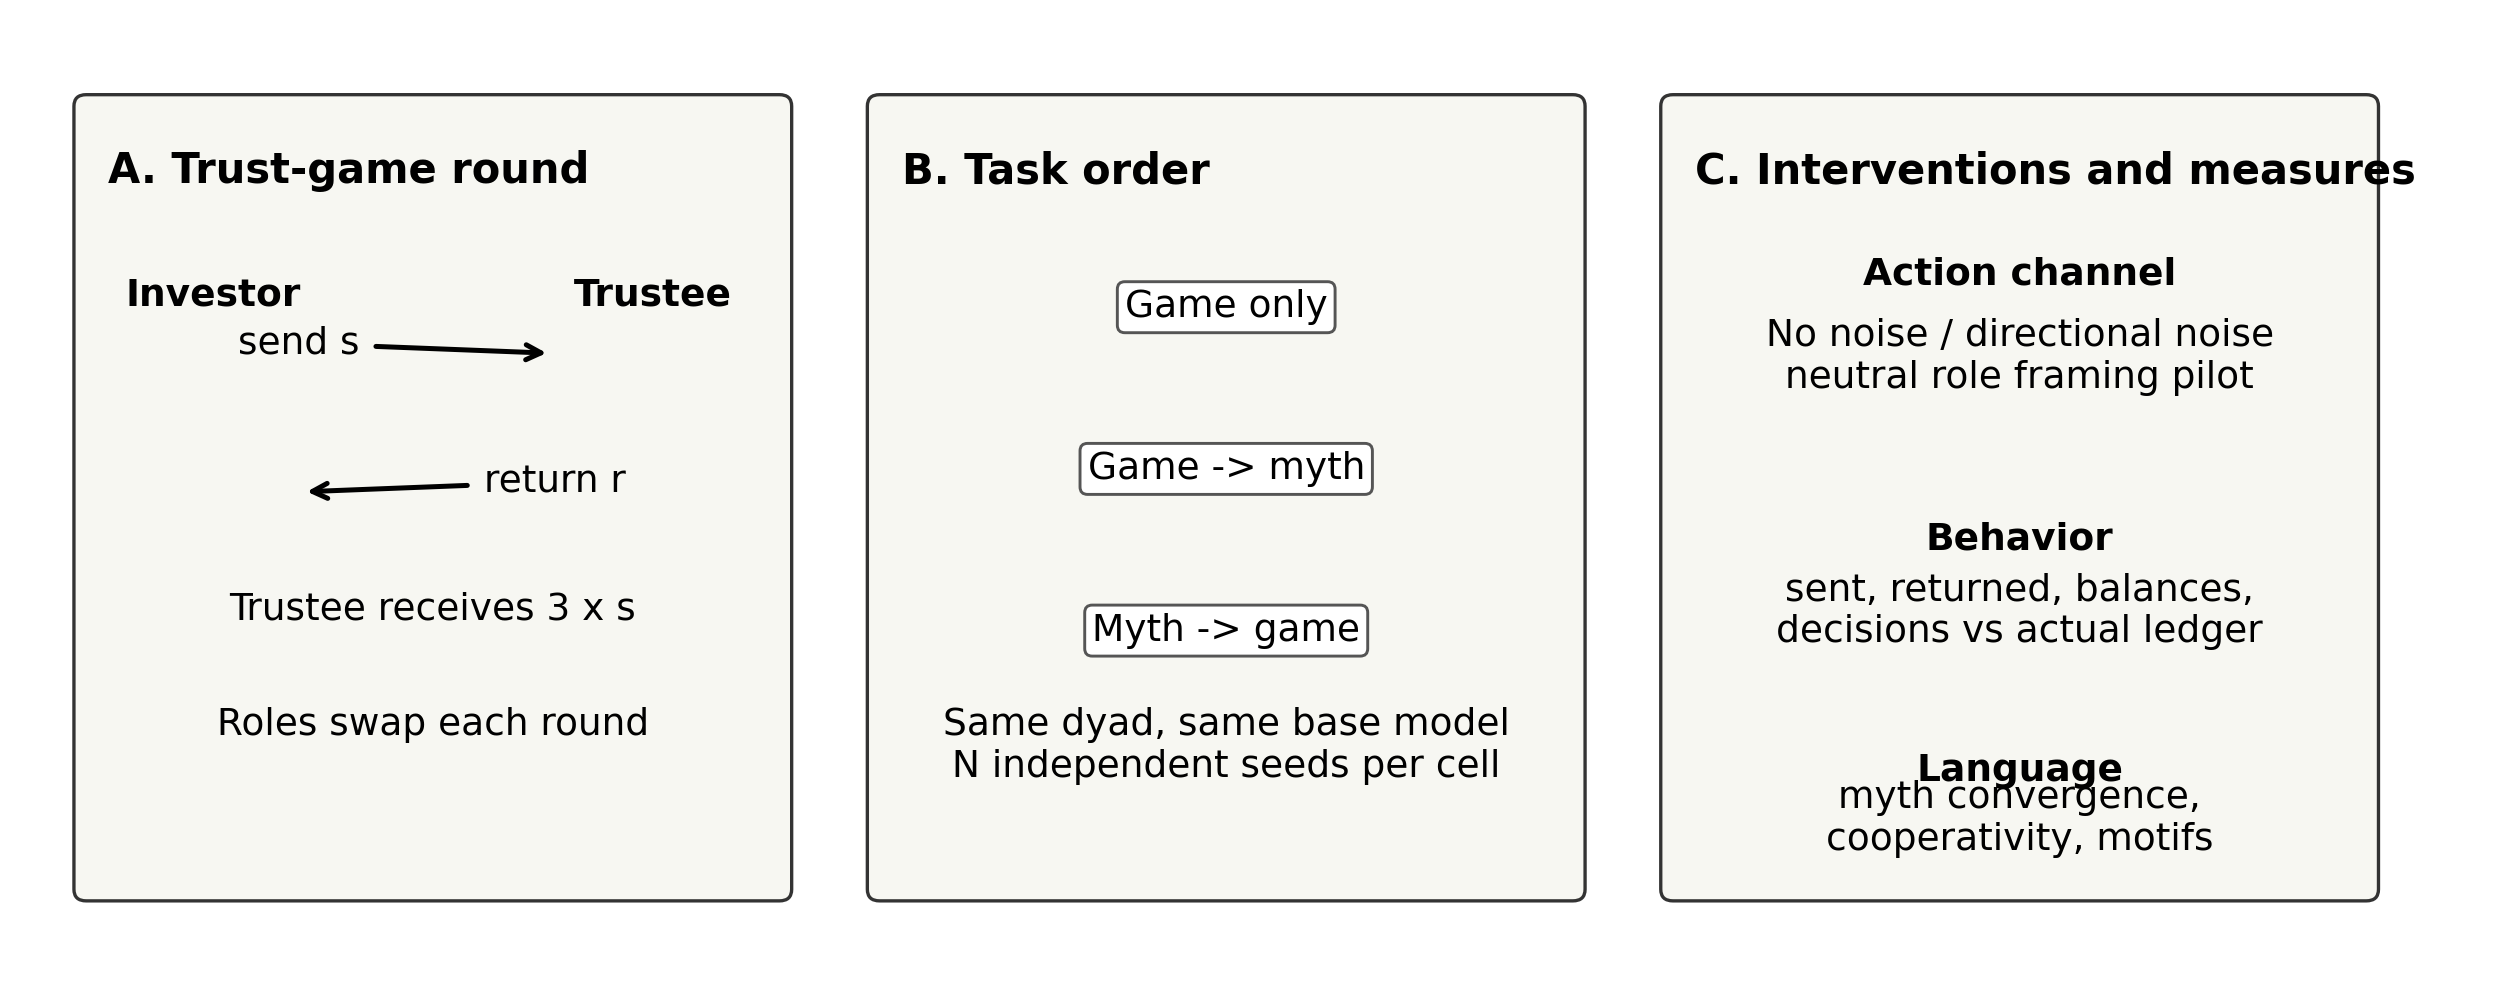
\includegraphics[width=1\linewidth,height=\textheight,keepaspectratio]{figures/fig1_design_schematic.png}

}

\caption{\label{fig-design}Experimental design. Two same-model agents
alternate investor and trustee roles in a repeated trust game. Runs
either contain only the game, interleave game before myth-writing, or
interleave myth-writing before the game. The action channel can be
unperturbed, directionally noised, or neutrally reframed; outputs
include both game ledgers and myth text.}

\end{figure}%

\subsection{3.2 Repeated trust game}\label{repeated-trust-game}

We use a role-swapping repeated Trust Game with endowment \(E = \$5\)
and multiplier \(m = 3\). Each game round has two sequential moves: the
investor chooses \(s_t \in [0, E]\) to send to the trustee; the trustee
receives \(3s_t\) and chooses \(r_t \in [0, 3s_t]\) to return. Per-round
payoffs are

\[
\pi^I_t = E - s_t + r_t,\qquad \pi^T_t = 3s_t - r_t.
\]

Roles alternate every game round, so both agents experience both sides.
Unless otherwise noted, runs use ten game rounds, temperature 0.8, a
neutral persona, and memory capacity three. The memory buffer is shared
across game and myth turns, so interleaving a myth task reduces the
number of recent game exchanges still visible in context. On the first
game round the investor sees only the rules and endowment; on later
rounds each agent is shown the previous round's sent, received, and
returned amounts, its payoff, and current cumulative balance.

\subsection{3.3 Myth-writing task}\label{myth-writing-task}

In myth-present conditions, each round also contains a creative-writing
turn. On the first myth round, both agents write a 200-word myth on the
unconstrained topic \texttt{anything}; on later rounds, each agent sees
its own previous myth and the partner's previous myth and is instructed
to adapt them in its own way. This creates a dyadic
iterated-transmission channel separate from the payoff-bearing game. The
game prompts never quote the partner's myth directly: cross-task
influence flows only through the shared message buffer, where the
agent's own prior myth and the partner myth it saw during writing remain
in recent context when later game decisions are made.

\subsection{3.4 Conditions}\label{conditions}

The main draft uses two direct-provider models: OpenAI
\texttt{gpt-5-nano} and Anthropic \texttt{claude-sonnet-4.5}. Gemini
pilot outputs are excluded from the main analysis as the run is
incomplete.

Task order has three game-containing levels: game-only, game then myth,
and myth then game. The main no-noise baseline is
\texttt{baseline\_v4\_mem3\_direct}, with 15 seeds per model and task
order. A neutral-framing pilot, \texttt{neutral\_framing\_v4\_pilot},
replaces investor/trustee wording with ROLE A/ROLE B allocation wording,
with three seeds per cell.

Noise is an environmental perturbation on the actual transfer ledger:
the model chooses a decision amount, the environment optionally perturbs
it, and the perturbed value is what arrives, enters payoffs, updates
balances, and appears in subsequent prompts. Unperturbed choices are
logged separately as \texttt{sent\_decision} and
\texttt{returned\_decision} (see §A.1 for full ledger bookkeeping). We
use three action-channel interventions. Directional uniform noise adds
\(\epsilon \sim \mathcal{U}(0,k)\) or
\(\epsilon \sim \mathcal{U}(-k,0)\) to both send and return actions and
clamps to range, with \(k=5\) for the completed manipulation-check runs.
Bootstrap noise replaces the returned amount with the maximum possible
return every round, an artificial reciprocity-support diagnostic. A
deterministic-max variant (every-round application of the maximum
perturbation) was run as a pilot but is under-replicated and excluded
from the main analysis (§A.4). Informed variants append a system-prompt
note flagging that transfers may be perturbed and that earnings reflect
arrived amounts.

Two further channel-design variants probe the cross-task mechanism
(results in §4.6). The \textbf{partner-myth injection} variant quotes
the partner's most recent myth verbatim inside the trust-game prompt,
opening a direct cross-task channel that the implicit design (§3.3)
keeps closed. The \textbf{forced-reasoning} variant adds a system-prompt
addendum requiring 2--3 sentences of reasoning before the JSON action,
used only with GPT-5-Nano to elicit the reasoning prose Claude emits by
default. Both variants run on all four bootstrap noise conditions;
partner-myth injection is also crossed with three myth-content
directions (neutral, cooperative, adversarial) for the §4.6 factorial.

\subsection{3.5 Measures and analysis}\label{measures-and-analysis}

Behavioural measures are computed from raw JSON states: final dyad
reward after ten game rounds, average sent and returned amounts (both
arrived and decision), return ratios, and per-cell dispersion across
seeds. The primary myth contrast is the median final-dyad-reward
difference between each myth-present task order and the matched
game-only cell within the same model and condition, with non-parametric
bootstrap percentile intervals over seeds. Each cell is then labelled by
a joint mean-shift × variance-ratio rule. The \(\Delta\)mean 95\% CI is
read as \emph{positive}, \emph{negative}, or \emph{null} (strictly
above, strictly below, or spanning zero); the myth-to-game
variance-ratio 95\% CI is read as \emph{consolidation},
\emph{destabilization}, or \emph{null} relative to one. The two axes
combine into \emph{lift+consolidation}, \emph{lift},
\emph{consolidation}, \emph{null}, \emph{harmful} (negative mean, null
variance), and \emph{destabilizing} (any other combination involving
negative mean or destabilization). Cells with \(n_{\text{myth}} < 10\)
are flagged \emph{missing} and excluded.

Linguistic measures span lightweight and embedding-based proxies, all
reproducible without API calls: cooperative-lexicon density, coarse
pronoun ratios, lag-1 cross-agent cooperativity correlations, and
dictionary-based coinage detection over the myth chain. We additionally
compute between-agent embedding cosine similarity per round using
\texttt{sentence-transformers/all-mpnet-base-v2} (normalized) and a
lexical proxy for myth content appearing in game-response prose: the
share of game-response tokens matching the agent's own preceding myth
vocabulary. LLM-judge similarity is deferred to follow-up analysis. All
manuscript tables and figures are generated from raw final JSON files
(see §A.2).

\section{4. Results}\label{results}

\subsection{4.1 Cross-model behavioural baselines
(no-noise)}\label{cross-model-behavioural-baselines-no-noise}

The two models occupy distinguishable but no longer dramatically
different no-noise regimes. In the v4 direct-provider configuration with
\(T = 10\), mem-3, and the unconstrained \texttt{anything} myth topic,
GPT-5-Nano reaches a mean cumulative dyad balance of 69.2 in the
game-only cell (median 71.0, std 4.6, \(N=15\)), with
\texttt{game\_myth} and \texttt{myth\_game} cells slightly higher (71.1
and 72.3). Claude-Sonnet-4.5's matched no-noise cell is under-replicated
(\(N = 2\)); the prior \texttt{baseline/} corpus gives a mean of 55.7
(median 55.0, std 2.6, \(N = 15\)). Maximum possible dyad reward is 150.
This revises an earlier working assumption: pilot work with GPT-5-Nano
via OpenRouter showed apparent floor-locking at mutual defection, but
with the direct provider the same model reaches roughly half the dyad
ceiling without any noise intervention. The cross-model gap is therefore
moderate, around 14 points, not the chasm the pilot suggested. We retain
Claude as the higher-cooperation regime and GPT-5-Nano as the more
variable one, but both exhibit substantive cooperation at baseline
\citep{serapio2023}. Across-seed dispersion drops
monotonically across task orders even at baseline (std 4.6 to 1.1 for
GPT-5-Nano), so the variance-reduction pattern in §4.3 is not specific
to the noise interventions.

\subsection{4.2 Effect of noise on the cooperation
profile}\label{effect-of-noise-on-the-cooperation-profile}

Direction of noise dominates the noise effect. Across the four
implemented mechanisms, positive (uniform \(+5\)) noise pushes both
models near the cooperation ceiling: Claude reaches a game-only mean of
73.5 (informed: 74.2), GPT-5-Nano 72.5 (informed: 72.4). Negative
(uniform \(-5\)) noise depresses Claude to 29.3 (informed: 30.4) but
lifts GPT-5-Nano relative to its baseline, to 37.9 (informed: 38.4);
agents perceive losses as smaller than they are, sustaining trust
longer.

Bootstrap noise is qualitatively distinct. It replaces the trustee's
returned amount with the maximum possible return every round, masking
actual reciprocation. GPT-5-Nano's game-only mean under bootstrap is
66.6 (informed: 67.9), well above no-noise. Bootstrap is therefore not
just an ``upward'' variant; it removes the trustee-return signal
entirely, a property that becomes load-bearing in §4.3. Informedness has
not produced a large qualitative shift: agents told the channel is noisy
still respond mainly to the realised ledger, and informed and uninformed
cells differ by 1--2 points across most cells. We treat it as a
robustness check. Gemini cells from the prior pilot are out of scope per
§3.4 and left for the EMNLP follow-up.

\subsection{4.3 Effect of myth-writing on game behaviour (the headline
question)}\label{effect-of-myth-writing-on-game-behaviour-the-headline-question}

The myth effect is conditional on the noise regime, not universal. Of 24
evaluable (model \(\times\) noise \(\times\) myth-order) cells in v4,
the joint \(\Delta\)mean and variance-ratio classification (with
bootstrap CIs) gives 4 lift+consolidation, 1 pure consolidation, 2 pure
lift, 13 null, 2 harmful, and 2 destabilizing --- seven positive cells,
four negative, thirteen null. Lift+consolidation lives entirely in
upward-noise cells; destabilization lives entirely in GPT-5-Nano
\(\times\) bootstrap. Figure~\ref{fig-decision} summarises the full
classification.

\begin{figure}

\centering{

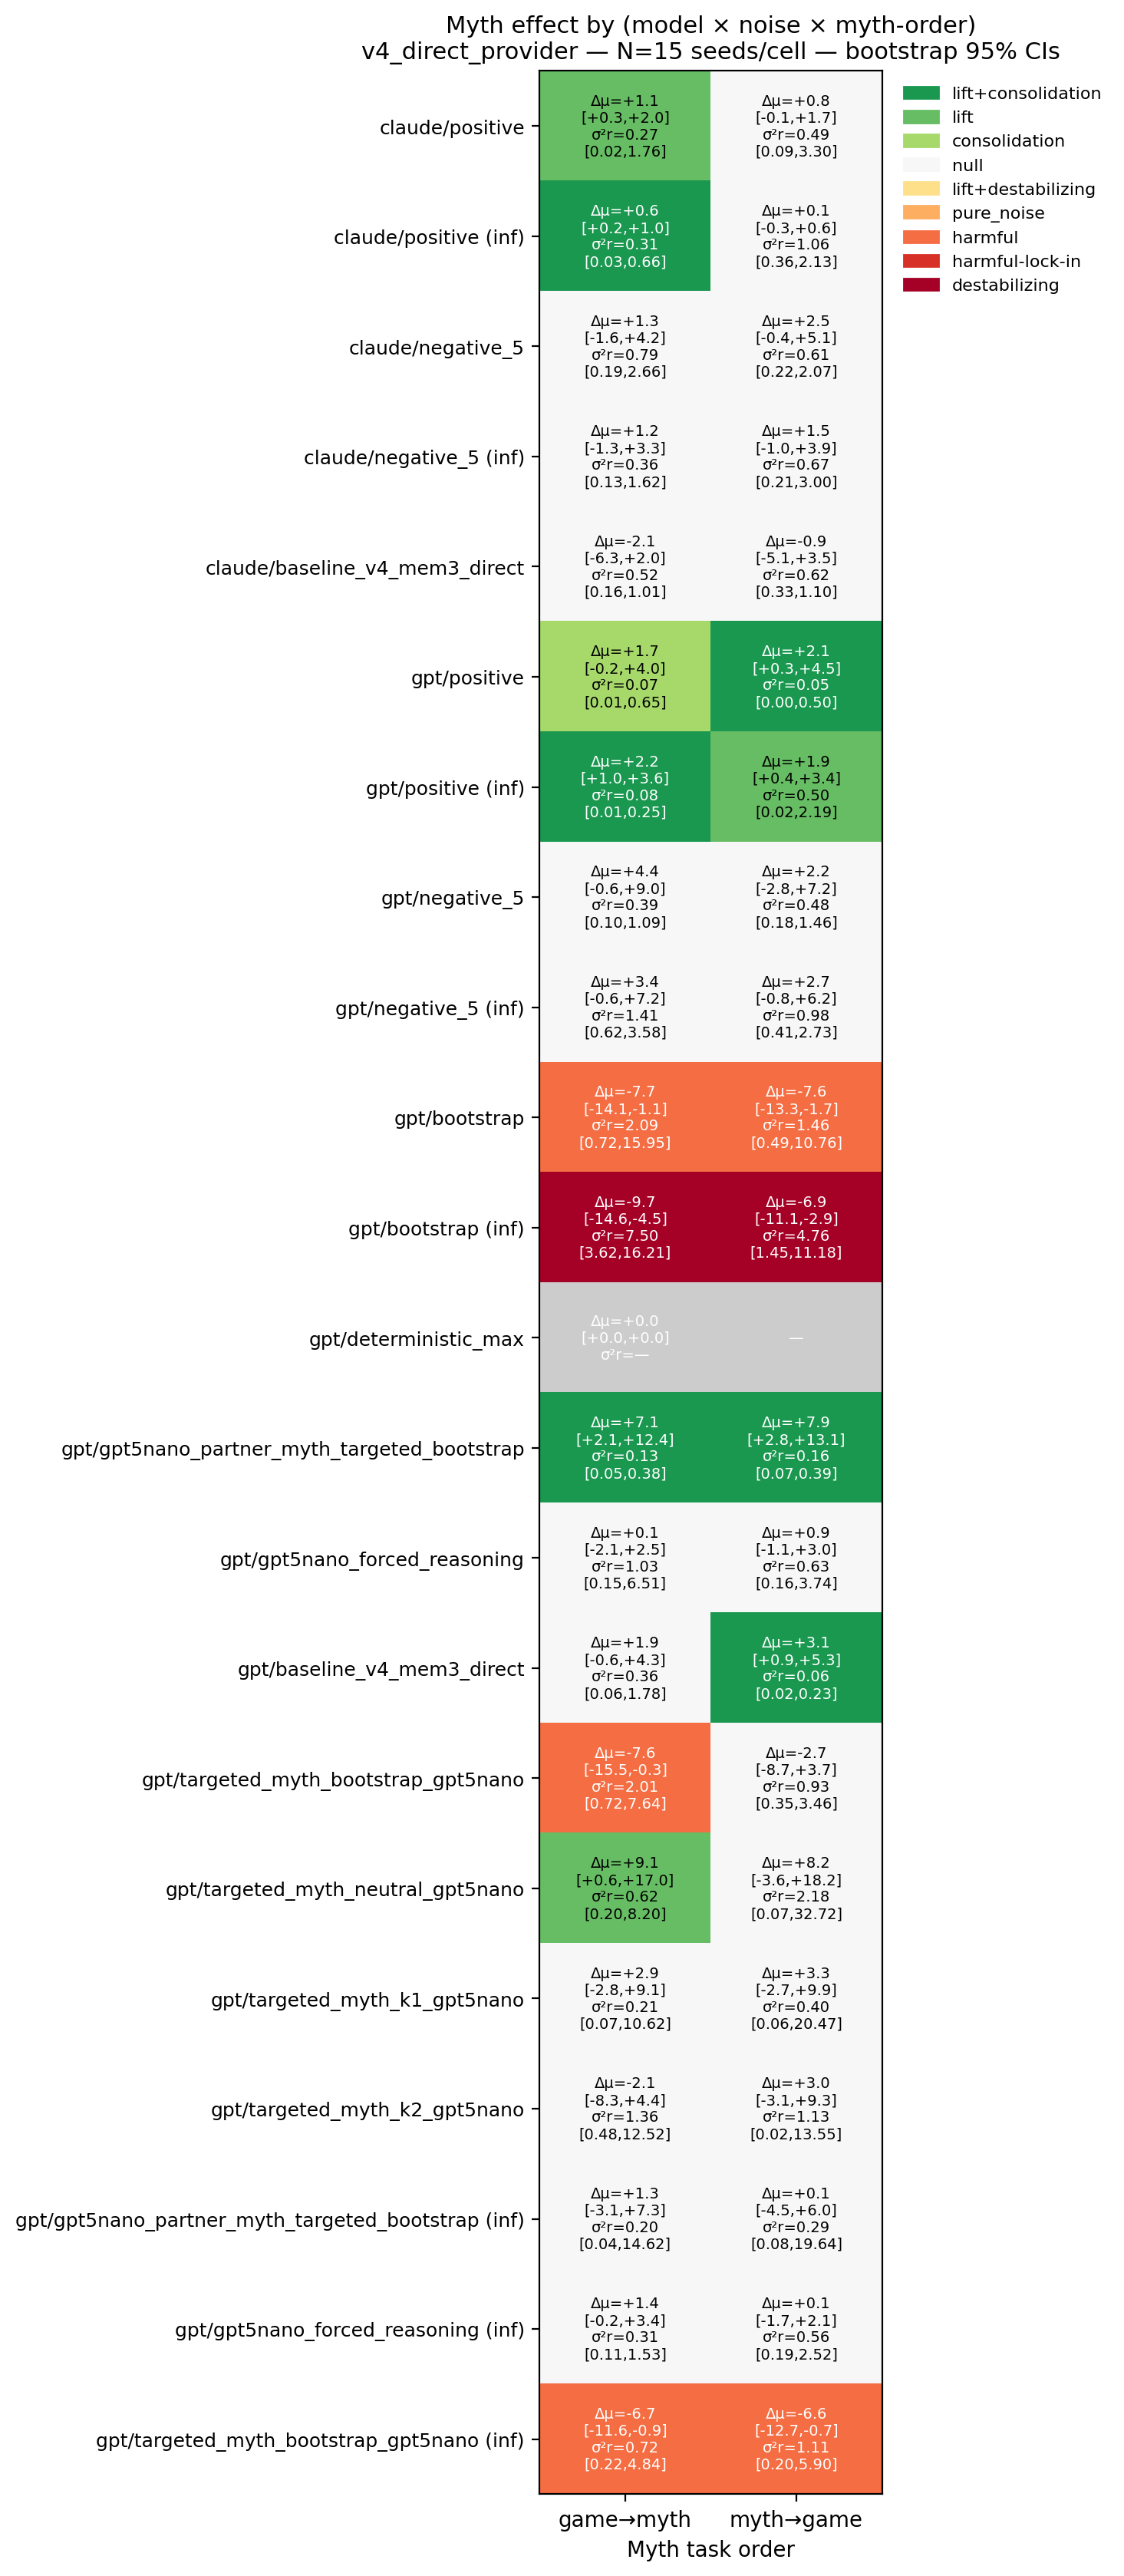
\includegraphics[width=1\linewidth,height=\textheight,keepaspectratio]{figures/fig_decision_table.png}

}

\caption{\label{fig-decision}3x3 classification (mean shift x variance
shift, bootstrap CIs) for every (model x noise x myth-order) cell. Green
= positive myth effect, red = negative, gray = null/missing.
Lift+consolidation lives in upward-noise cells; destabilization in
GPT-5-Nano x bootstrap.}

\end{figure}%

The strongest positive cells (lift+consolidation, with both mean and
variance CIs strict) sit entirely in upward-noise conditions, and their
variance reductions run between 3\(\times\) and 20\(\times\) relative to
the matched game-only cell. The negative cells, by contrast, are all
GPT-5-Nano \(\times\) bootstrap; the four harmful or destabilizing cells
share \(\Delta\)mean estimates roughly between \(-7\) and \(-10\) points
of dyad reward. Per-cell estimates and bootstrap CIs are tabulated in
Table~\ref{tbl-percell-deltas} (§A.4).

The asymmetry is structural. Under upward noise, agents observe a
perceived signal at least as positive as the underlying decision, and
the dyad locks onto a coordination point \citep{boyd2011}. Under
bootstrap, the perceived signal contradicts the underlying interaction
and myth introduces a competing structured prior. All eight
negative-noise cells are null.

\begin{figure}

\centering{

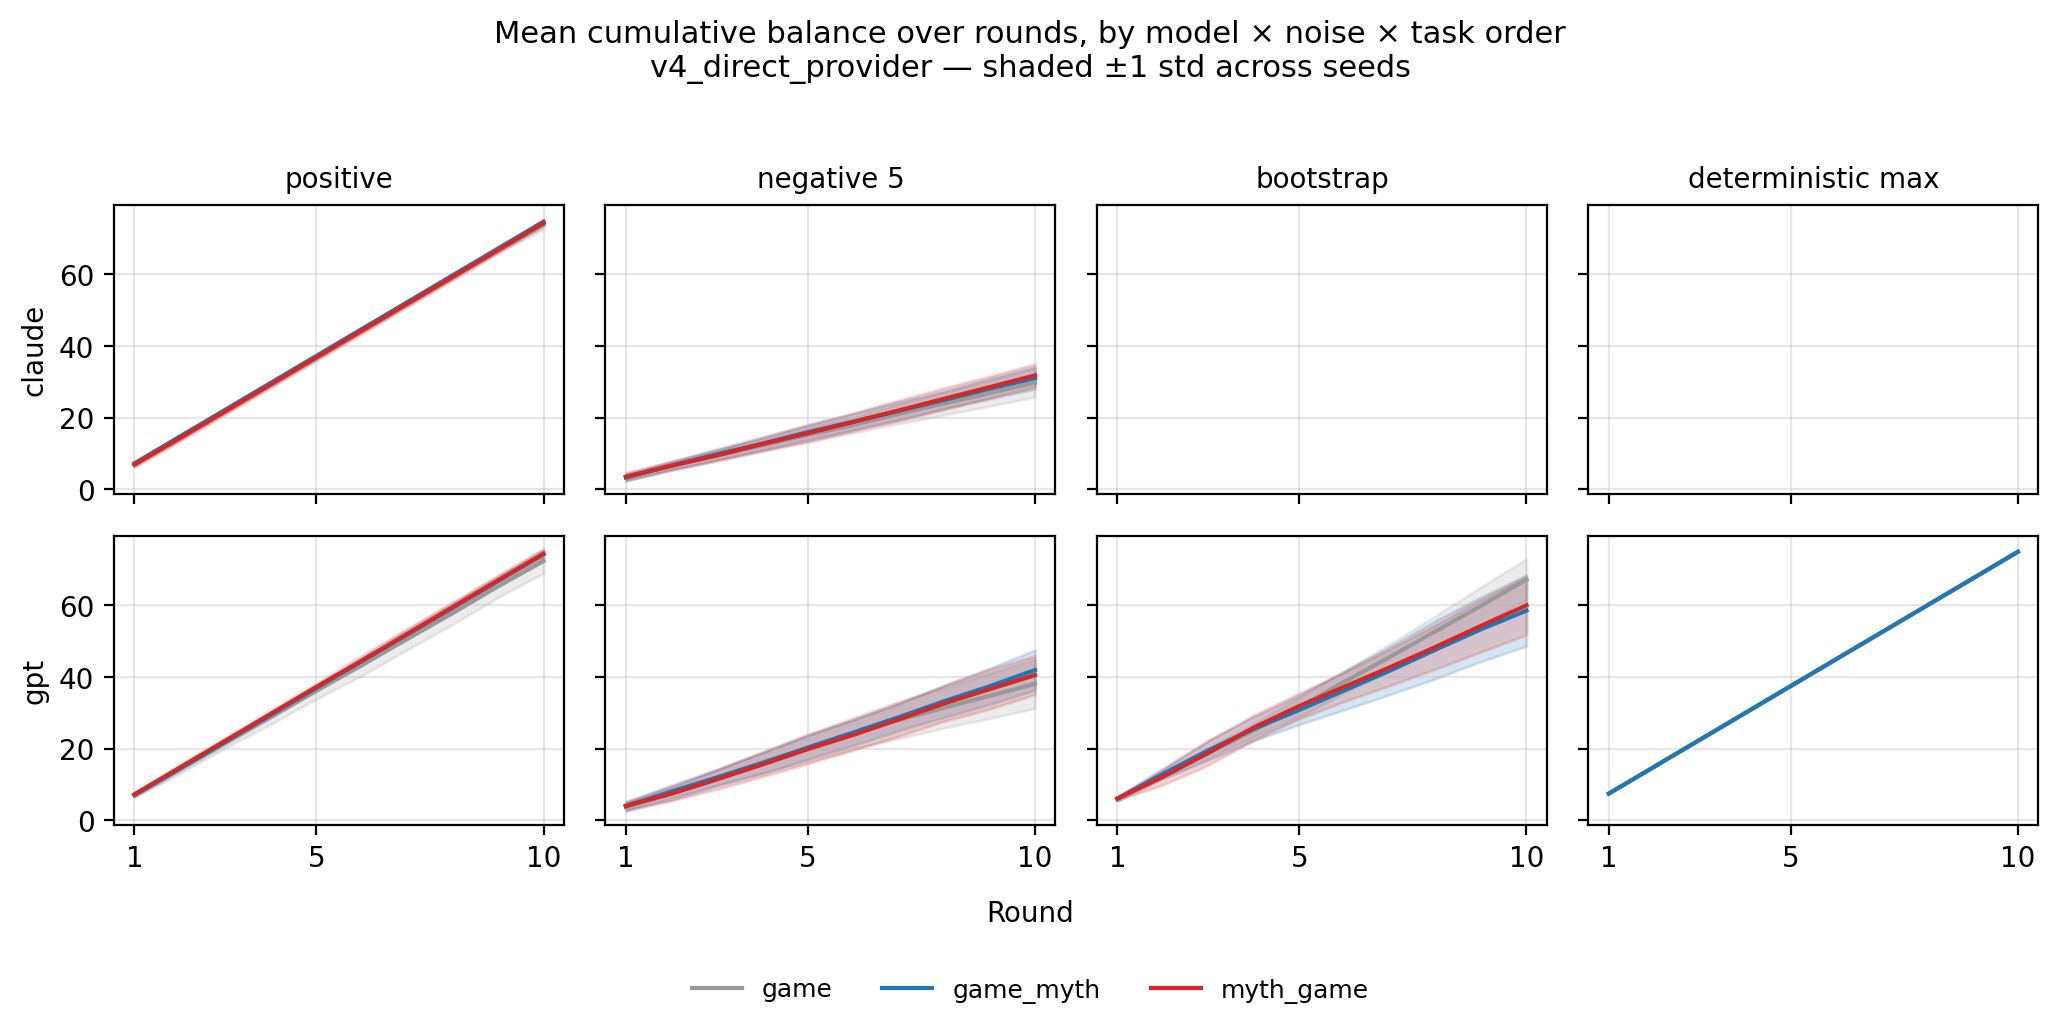
\includegraphics[width=1\linewidth,height=\textheight,keepaspectratio]{figures/fig_trajectories.png}

}

\caption{\label{fig-trajectories}Mean cumulative balance over rounds,
faceted by (model x noise) with one line per task order. Shaded ribbons
are +/-1 std across seeds. The bootstrap-noise harm pattern is visible
in the bottom row: gray (game-only) sits above blue/red (myth-present).}

\end{figure}%

\subsection{4.4 Linguistic dynamics in the myth
chain}\label{linguistic-dynamics-in-the-myth-chain}

Between-agent embedding cosine convergence is robust across cells.
Pairwise cosine between Agent\_1 and Agent\_2 myths at the same round
(sentence-transformers/all-mpnet-base-v2, normalised) shows a positive
slope in 18 of 21 cells, strongest in GPT-5-Nano \(\times\) negative\_5
\(\times\) \texttt{myth\_game} (slope +0.027/round {[}0.016, 0.038{]},
cosine 0.42 \(\rightarrow\) 0.74 across 10 rounds), GPT-5-Nano
\(\times\) bootstrap \(\times\) \texttt{myth\_game} (+0.023/round), and
Claude \(\times\) positive (informed) \(\times\) \texttt{myth\_game}
(+0.021/round). Convergence holds even where the game outcome is null or
harmful, so linguistic alignment is not contingent on behavioural
improvement \citep{fontana2024}.

Lag-1 cross-agent cooperativity correlations are positive in every cell.
Pearson r between Agent\_A's cooperativity-lexicon score in round-\(t\)
myth and Agent\_B's in round \(t+1\) ranges 0.27--0.58 in mean per-dyad
max-direction, with 27--73\% of dyads above \textbar r\textbar{}
\textgreater{} 0.5. The strongest cell is GPT-5-Nano \(\times\) positive
(informed) \(\times\) \texttt{myth\_game} (lag1\_max mean 0.58 {[}0.43,
0.71{]}, 73\% of dyads above 0.5); the pilot's Claude r \(\approx\) 0.72
sits at the upper tail of a clearly non-zero distribution and is
representative, not anomalous. Both convergence and lag-1 transmission
are summarised across cells in Figure~\ref{fig-linguistic}.

Coinages persist within myth chains but do not transfer into
game-reasoning text in any cell; the pilot observation of cross-task
coinage leakage does not replicate at corpus scale.

\begin{figure}

\centering{

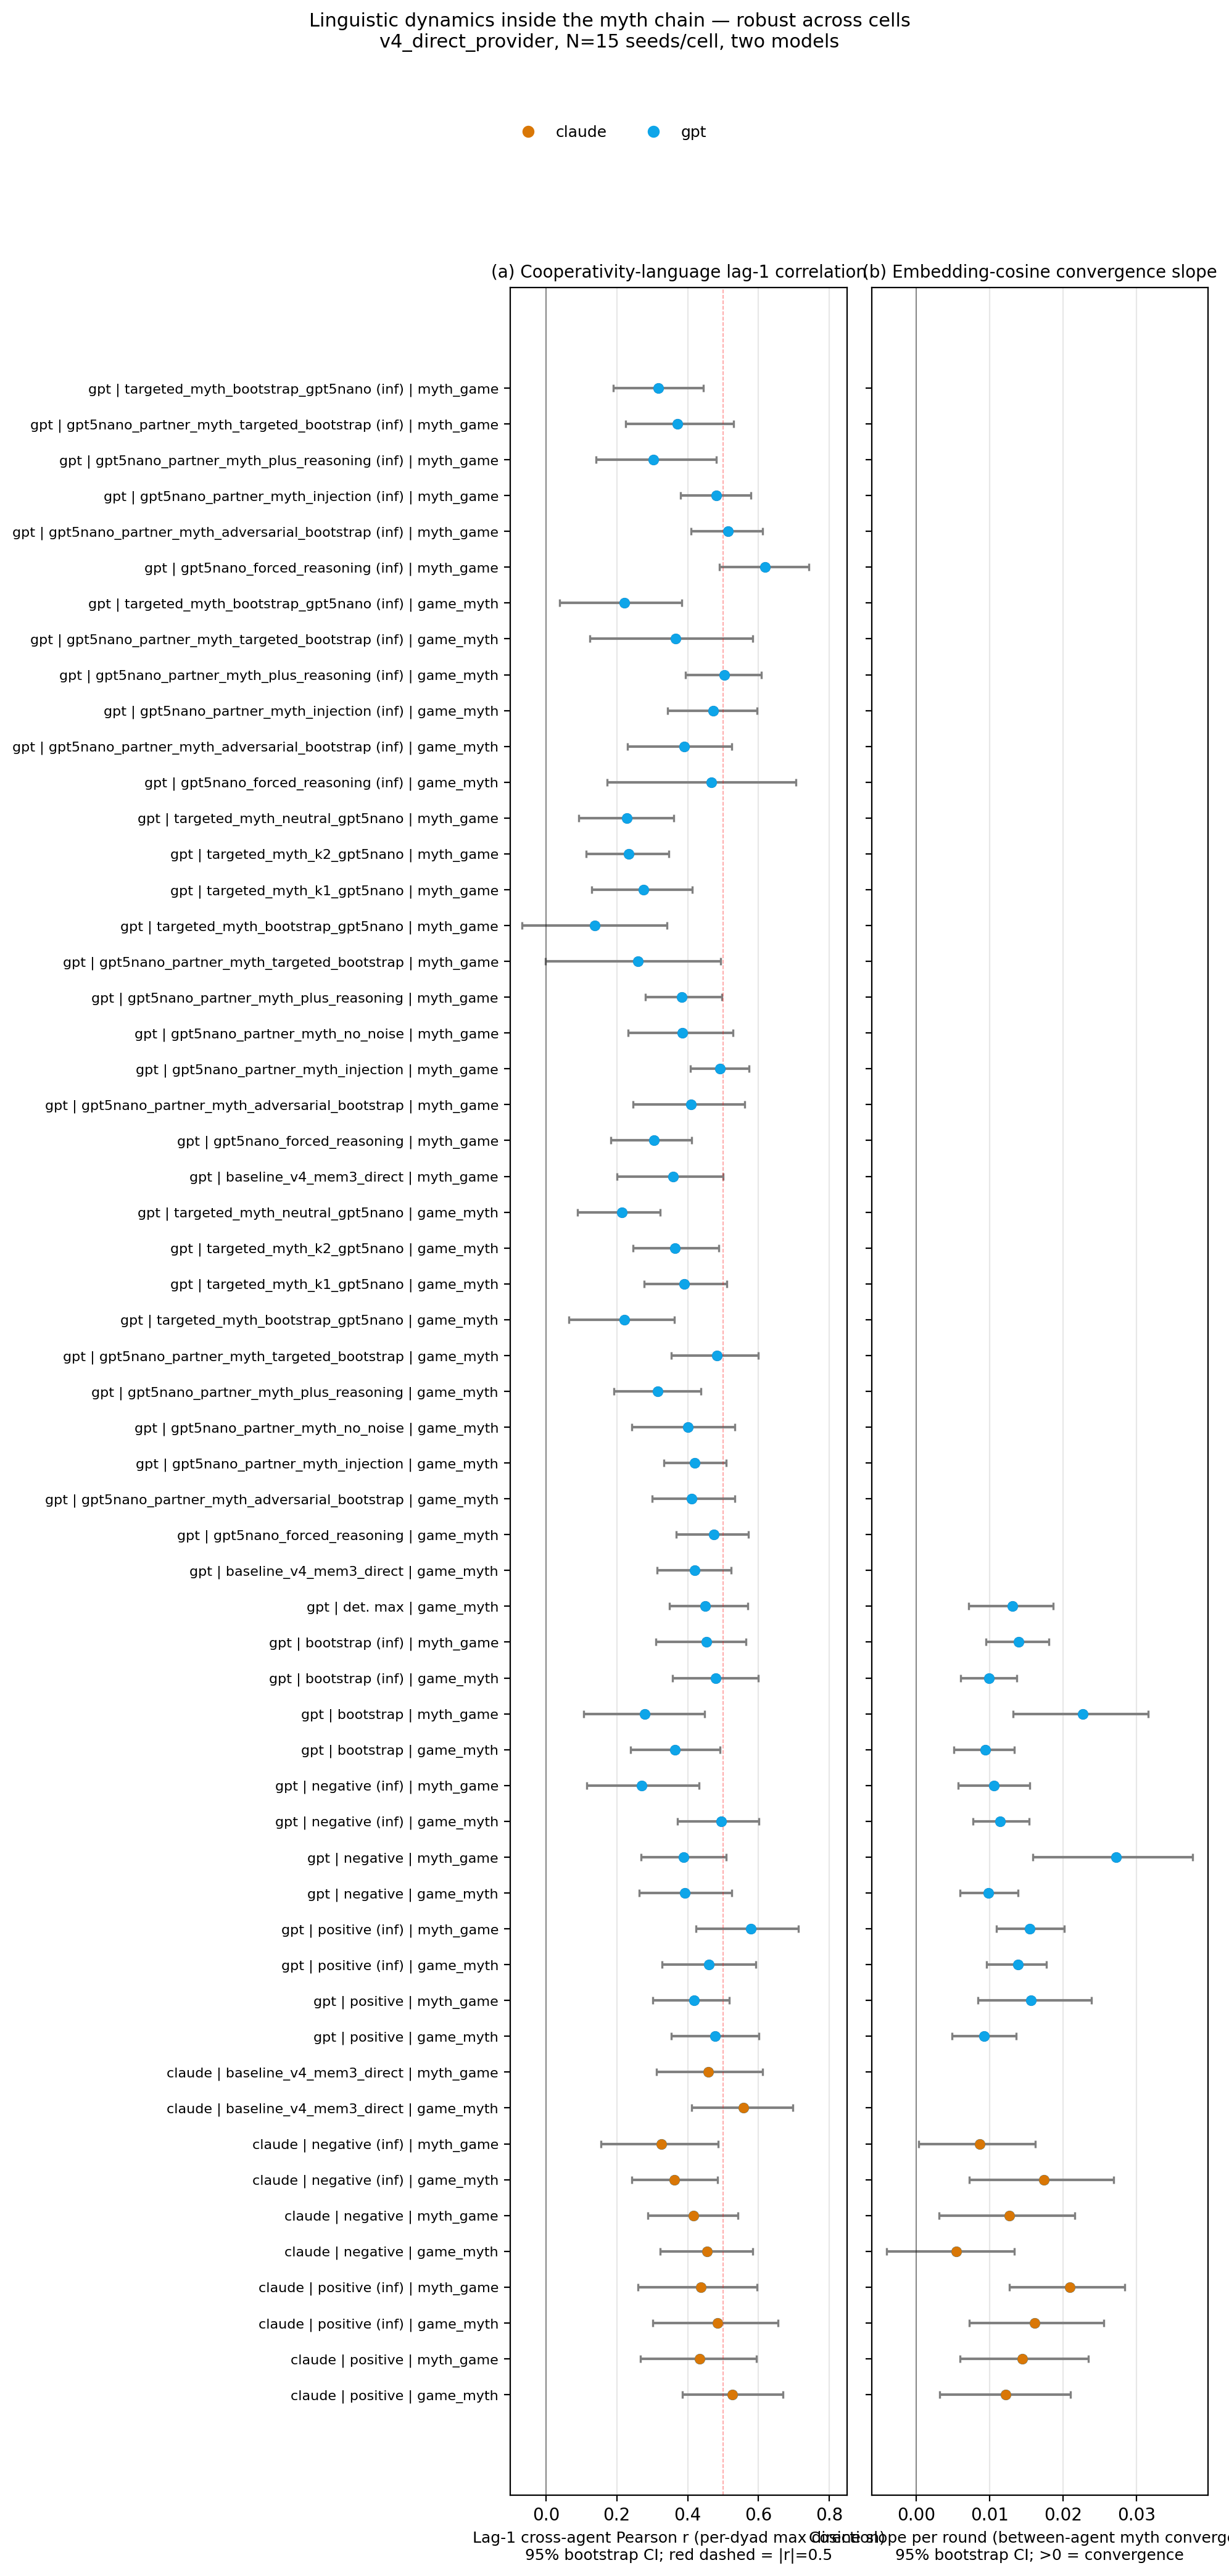
\includegraphics[width=1\linewidth,height=\textheight,keepaspectratio]{figures/fig_linguistic_dynamics.png}

}

\caption{\label{fig-linguistic}Lag-1 cross-agent cooperativity
correlation (left) and embedding-cosine convergence slope (right) across
all (model x noise x myth-order) cells, with Claude and GPT-5-Nano
overlaid.}

\end{figure}%

\subsection{4.5 Coupling between game behaviour and myth
content}\label{coupling-between-game-behaviour-and-myth-content}

Claude emits extensive game-response prose threaded with own-myth
vocabulary: 78--82\% of round-level responses contain at least one
content word from the preceding myth (mean 5--7 unique overlaps per
response), and 100\% of runs have at least one such reference, with
theme-lexicon hits (story, spirit, elder, sacred, ancestor, ritual)
reaching 10--33\% of responses. GPT-5-Nano, by default, emits no
reasoning prose at all --- its \texttt{game\_responses{[}ag{]}.content}
is the bare JSON action (e.g.~\texttt{\{"send":\ 3\}}, \textasciitilde12
characters), which makes the metric methodologically undecidable in that
configuration. An A3 forced-reasoning addendum closes the gap:
GPT-5-Nano under A3 matches Claude's any-hit rate at 80--82\%
(Figure~\ref{fig-reason-coding}).

\begin{figure}

\centering{

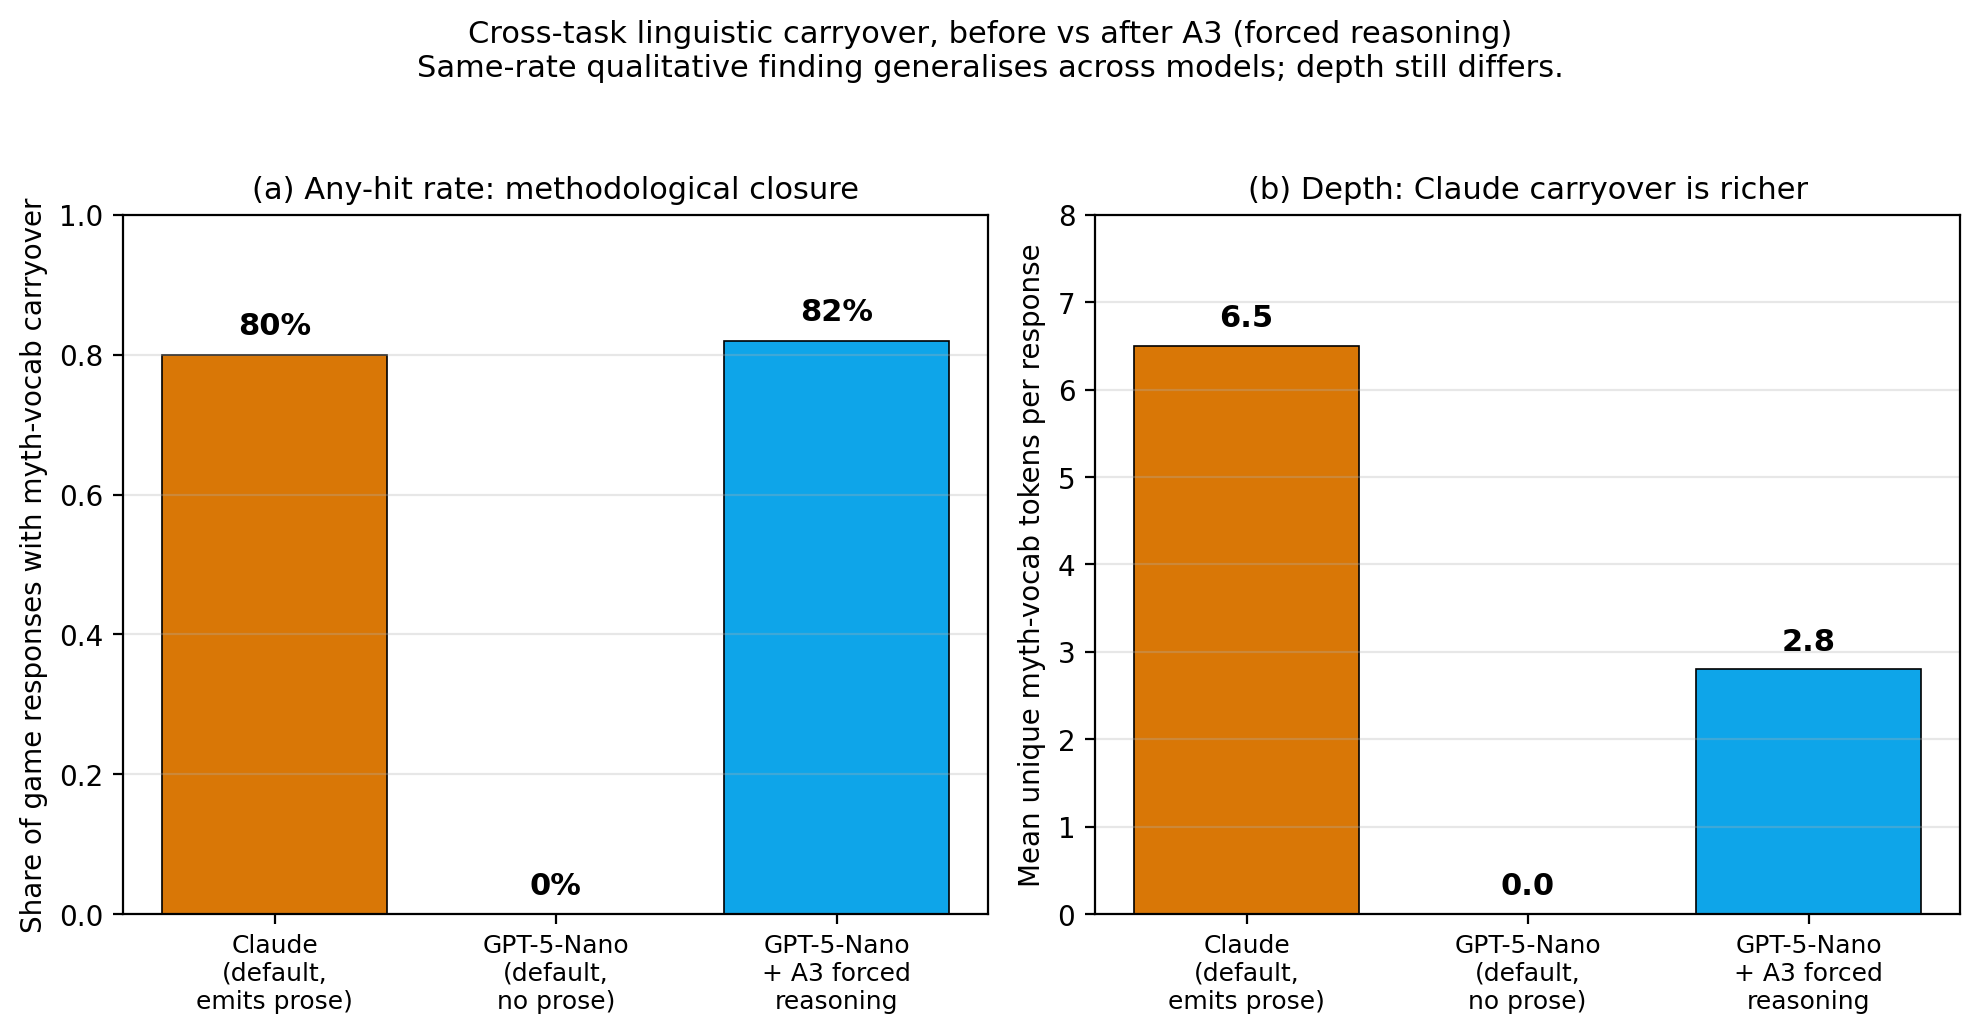
\includegraphics[width=1\linewidth,height=\textheight,keepaspectratio]{figures/fig_reason_coding_updated.png}

}

\caption{\label{fig-reason-coding}Any-hit rate (left) and depth (right)
of own-myth-vocabulary carryover into game responses, comparing Claude
default, GPT-5-Nano default, and GPT-5-Nano under A3 forced reasoning.}

\end{figure}%

Three layers of evidence point the same direction: between-agent
embeddings systematically converge in 18/21 cells; cooperativity-lexicon
scores transmit lag-1 between agents in every cell; and for Claude,
myth-vocabulary content is present in essentially every game response.
The carriers differ across semantic embedding, narrow lexical scoring,
and thematic vocabulary, but all three indicate that the myth channel is
doing measurable work \citep{leng2023, piatti2024}.
The §4.3 mean-and-variance picture is consistent with this: language is
doing real work, but its sign depends on whether it converges with or
competes against the noise channel \citep{smith2017}.

\subsection{4.6 Tightening the cross-task channel --- a 2x3 mechanism
factorial}\label{tightening-the-cross-task-channel-a-2x3-mechanism-factorial}

We opened the implicit channel of §3.3 by quoting the partner's most
recent myth verbatim inside the trust-game prompt --- a
\textbf{partner-myth injection} variant --- and ran it on the four noise
conditions of §4.3 (all GPT-5-Nano).

In the bootstrap cells where myth was harmful, partner-myth injection
reverses the destabilisation. Bootstrap \(\times\) \texttt{game\_myth}:
baseline anything-myth \(\Delta\)mean -7.7 against a game-only mean of
58.9 (std 11.0); with injection, \(\Delta\)mean +1.5 (mean 68.1, std
3.5). The pattern holds in \texttt{myth\_game} (\(\Delta\)mean -7.6
\(\rightarrow\) +1.8; std 9.2 \(\rightarrow\) 3.6). Across-seed variance
collapses roughly threefold and mean cooperation returns to baseline. In
the positive-noise cells where myth was already lifting, injection adds
no detectable extra effect (\(\Delta\)mean change \textless{} 0.2 across
all four positive cells). The intervention is regime-conditional: it
acts only where the implicit channel was failing.

To discriminate visibility from content, a follow-up factorial varied
the myth topic across three directions: anything-myth (neutral content),
cooperative-themed (\texttt{reciprocity\_oath}, a story about honouring
reciprocal obligations), and adversarial
(\texttt{trickster\_exploitation}, a story about being exploited by a
defector). Each crossed with the visibility manipulation (no injection
vs injection), yielding {[}N\_CELLS{]} cells of fresh data, all
GPT-5-Nano \(\times\) bootstrap, \(N = 15\) per cell.

Visibility dominates content direction. The 2 \(\times\) 3 factorial on
bootstrap \(\times\) \texttt{game\_myth} (uninformed):

{\def\LTcaptype{none} % do not increment counter
\begin{longtable}[]{@{}
  >{\raggedright\arraybackslash}p{(\linewidth - 4\tabcolsep) * \real{0.3333}}
  >{\raggedright\arraybackslash}p{(\linewidth - 4\tabcolsep) * \real{0.3333}}
  >{\raggedright\arraybackslash}p{(\linewidth - 4\tabcolsep) * \real{0.3333}}@{}}
\toprule\noalign{}
\begin{minipage}[b]{\linewidth}\raggedright
Content / visibility
\end{minipage} & \begin{minipage}[b]{\linewidth}\raggedright
No injection
\end{minipage} & \begin{minipage}[b]{\linewidth}\raggedright
+ Injection
\end{minipage} \\
\midrule\noalign{}
\endhead
\bottomrule\noalign{}
\endlastfoot
Anything (neutral) & 58.9 \(\pm\) 11.0 (harmful) & \textbf{68.1 \(\pm\)
3.5} (rescue) \\
Cooperative & 57.4 \(\pm\) 12.4 (harmful) & \textbf{69.8 \(\pm\) 2.9}
(rescue) \\
Adversarial (defection-themed) & n/a & \textbf{66.6 \(\pm\) 5.5}
(rescue) \\
\end{longtable}
}

(The adversarial \(\times\) no-injection cell was not run; the
no-injection harm pattern was already established in the neutral and
cooperative arms.) All three injection cells land in the rescue zone
(66--70); both no-injection cells stay in the harmful zone
(\textasciitilde58). The same pattern recurs in \texttt{myth\_game} and
in the informed bootstrap variants. Cooperative content modulates the
rescue marginally upward (\textasciitilde+2 over neutral) and
adversarial content marginally downward (\textasciitilde-2); content
direction explains less than 5\% of variance, visibility the rest
(Figure~\ref{fig-bootstrap-rescue}).

\begin{figure}

\centering{

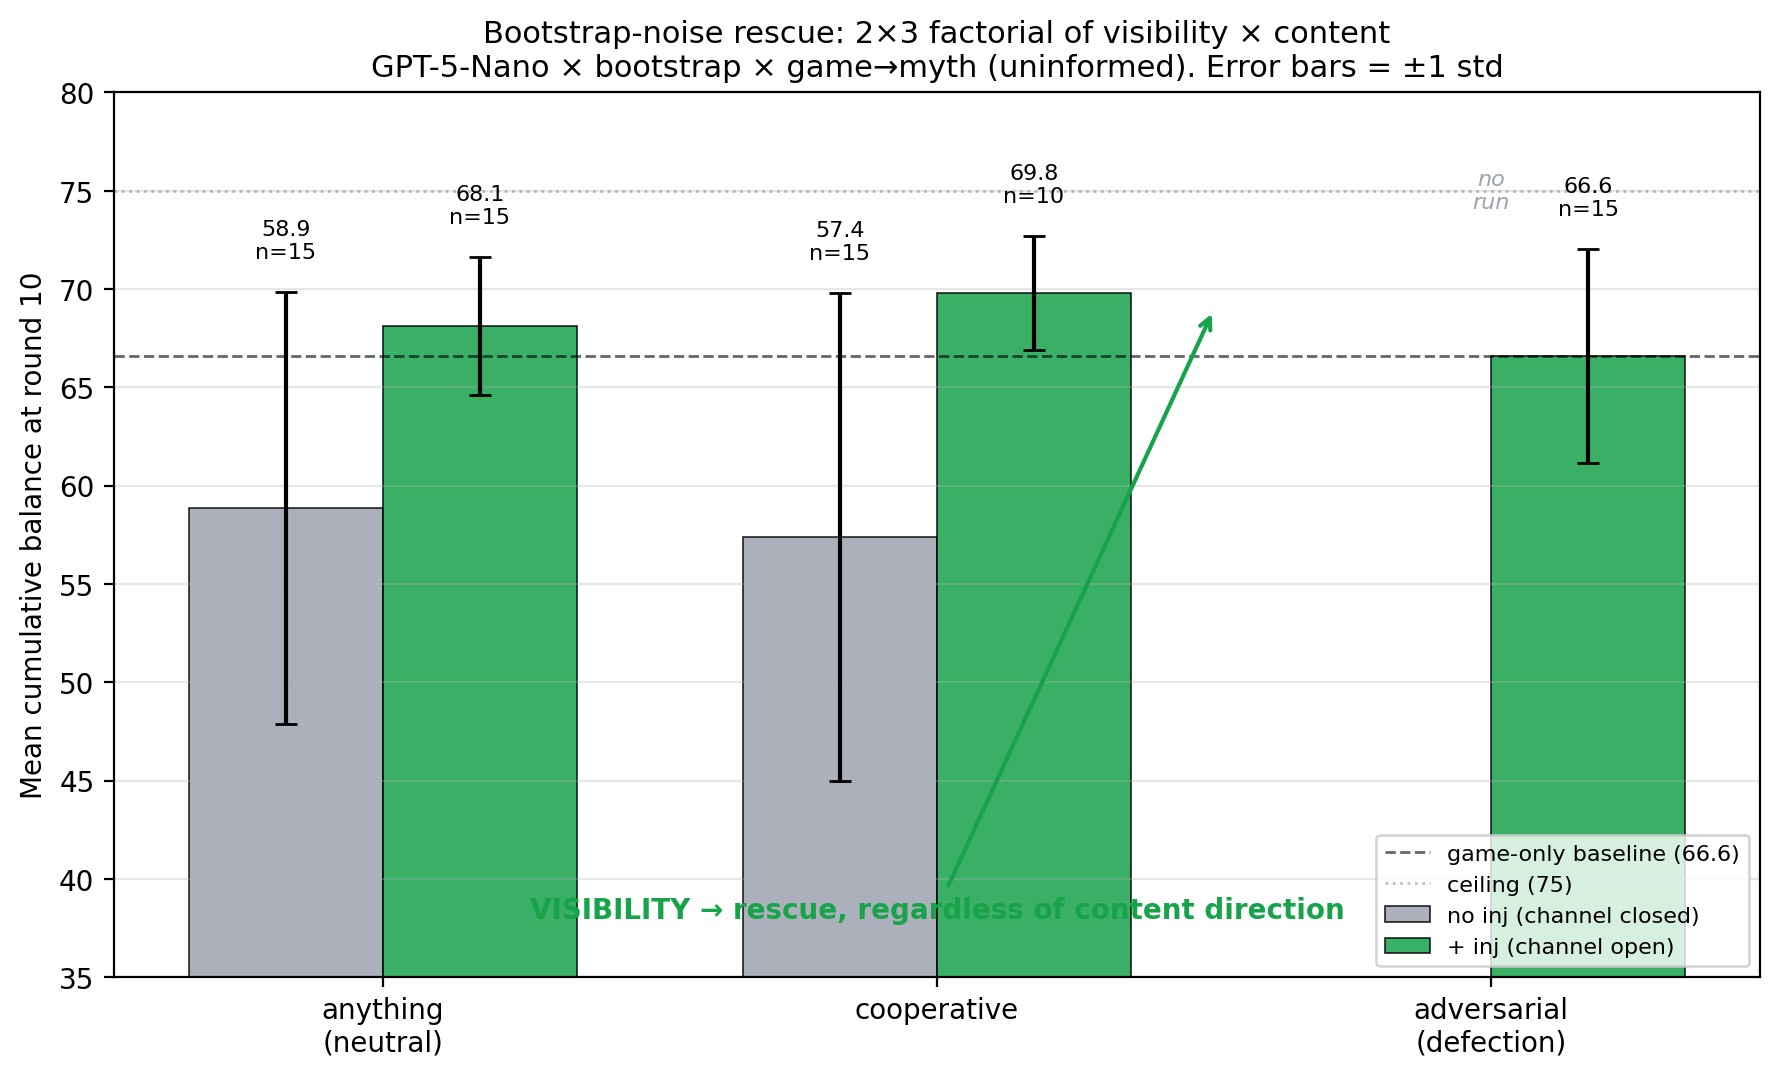
\includegraphics[width=1\linewidth,height=\textheight,keepaspectratio]{figures/fig_bootstrap_rescue.png}

}

\caption{\label{fig-bootstrap-rescue}Bootstrap-noise rescue under
partner-myth visibility for GPT-5-Nano x bootstrap x game\_myth
(uninformed): visibility produces the rescue across all three content
directions, with content direction modulating the rescue only
marginally.}

\end{figure}%

Two further controls anchor the mechanism. An A1 \(\times\) no-noise
baseline produces no effect (\(\Delta\)mean -0.8 to +0.9 across two
cells, \(N = 30\) runs, 0 failures), ruling out the alternative that
injection simply lifts cooperation by adding more partner-related text;
if that were the mechanism, no-noise cells would also lift. An A1+A3
combination (injection plus a system-prompt addendum requiring 2--3
sentences of reasoning before each JSON action) erases A1's rescue in
the bootstrap cells (\(\Delta\)mean returns to \textasciitilde-13
against A1). Inspection shows GPT-5-Nano with forced reasoning surfaces
explicit cost--benefit calculation rather than coordination; ``net zero
last round \(\rightarrow\) send less'' patterns dominate. The Claude
reasoning-prose carryover from §4.5 may therefore be partly
correlational: cooperative reasoning correlates with cooperative
behaviour without necessarily causing it \citep{vallinder2024}.

We read the mechanism as follows. Under bootstrap, agents see a
perceived signal that contradicts the underlying game; with the
partner's myth visible, both have common-knowledge access to a shared
narrative anchor and resolve the contradiction by coordinating on it
\citep{chwe2001}. Cooperative content provides a modest amplifier and
adversarial content does not subtract enough to break the rescue, so
content is a small modulator and visibility carries the work; the
competing-prior interpretation is falsified by both content arms
(cooperative and adversarial), since visibility rescues regardless of
direction.

\section{5. Discussion}\label{discussion}

\subsection{5.1 What we found and what we
didn't}\label{what-we-found-and-what-we-didnt}

The corpus yields three layered findings. Cross-model variation in
baseline cooperation is moderate, around 14 points of dyad reward, but
its direction depends on the noise regime: in the matched no-noise
corpus GPT-5-Nano is somewhat above Claude, under positive noise both
models reach the cooperation ceiling, and under negative noise
GPT-5-Nano sustains higher cooperation than Claude (§4.1--4.2). The
myth-writing effect on game payoffs is heterogeneous and conditional on
noise: of 24 evaluable (model \(\times\) noise \(\times\) myth-order)
cells, seven are positive, four are negative, and thirteen are null
(§4.3). Linguistic dynamics inside the myth chain are robust regardless
of behavioural outcome: between-agent embedding cosine converges in 18
of 21 cells, lag-1 cross-agent cooperativity correlations are positive
in every cell, and Claude's game-response prose threads its own myth
vocabulary into roughly four-fifths of rounds (§4.4--4.5).

About half of cells show no detectable myth effect on mean cumulative
reward, and we report this as the central empirical fact rather than
burying it. The §1 question was whether language between LLM agents is
\emph{load-bearing} on cooperation; the data answer ``yes, but
conditionally and asymmetrically.'' Where the noise regime gives the
dyad headroom and the perceived signal is useful, myth-writing produces
a small mean lift and a 3\(\times\) to 20\(\times\) drop in across-seed
dispersion in the strongest cells. Where the noise regime systematically
contradicts the action signal, it actively harms cooperation. The narrow
form of the §1 thesis survives; the broader form, a uniform cooperation
lift, is rejected.

\subsection{5.2 The active mechanism is common-knowledge visibility, not
content
semantics}\label{the-active-mechanism-is-common-knowledge-visibility-not-content-semantics}

The §4.3 mean-and-variance pattern admits multiple mechanism candidates,
and the §4.6 factorial decomposes between them. Three candidates
motivated the follow-up: myth as a \emph{competing structured prior}
whose narrative content competes with the noise channel; myth as a
\emph{cooperative-content cue} whose semantics directly guide
cooperation; and myth as a \emph{common-knowledge anchor} in the sense
of Chwe \citep{chwe2001}, where both agents seeing the same narrative
creates a shared reference that resolves the noise channel's
contradictions. Under a visibility \(\times\) content factorial, the
first predicts that more visible myth makes things worse, the second
that cooperative content rescues whether or not it is shared, and the
third that visibility rescues regardless of content direction.

The data support the third candidate and falsify the first two.
Visibility dominates content direction: common-knowledge injection
rescues bootstrap cells whether content is neutral, cooperative, or
adversarial, with content modulating an order of magnitude less (cell
means and stds in §4.6 and Figure~\ref{fig-bootstrap-rescue}). Two
controls anchor the reading. The same injection produces no detectable
effect at no-noise baseline, ruling out a generic-text-lift alternative;
the intervention is regime-conditional. Adding forced reasoning prose on
top of injection (A1+A3) erases the rescue, with GPT-5-Nano surfacing
cost--benefit reasoning that depresses cooperation below the
no-injection baseline. This complicates the §4.5 prose-carries-content
reading and suggests Claude's higher cooperation may be partly substrate
(Claude-as-cooperator) rather than carryover.

Stated as a falsifiable claim: under bootstrap-style noise, agents
observe a perceived reciprocation signal that systematically contradicts
their own game-math; with both agents' previous narrative writing made
common-knowledge in the game prompt, both have access to the same shared
reference and resolve the contradiction by coordinating on it. The
shared reference is the active ingredient; its semantic direction is a
small modulator. This is consistent with the cultural-evolution
literature on narrative as a coordination device \citep{boyd2011, chwe2001}: narratives stabilise cooperation by being publicly
shared, not primarily by being prescriptively cooperative.

\subsection{5.3 Cross-model variation, narrowed
honestly}\label{cross-model-variation-narrowed-honestly}

The submitted scope is a two-model claim: the v4 direct-provider corpus
contains Claude and GPT-5-Nano, with Gemini cells deferred to a re-run
under the corrected noise pipeline. The two models are distinguishable
in mean cooperation (\textasciitilde14 points of dyad reward at
no-noise, §4.1) but both reach near-ceiling cooperation under positive
noise. Cross-model variation in social-game behaviour is a recurring
finding \citep{fontana2024, leng2023, serapio2023}; our contribution is more specific in that variation
persists \emph{under matched experimental conditions} and shows up not
only in mean cooperation but in the very different shapes of the
linguistic channel. Claude emits extensive game-response prose threaded
with own-myth vocabulary; GPT-5-Nano emits only the structured action
with no surrounding prose at all (§4.5). Pooling across frontier models
would have hidden both the bootstrap-noise harm pattern
(GPT-5-Nano-only) and the reasoning-prose presence (Claude-only); future
LLM-game work should report findings with model-stratified statistics.

\subsection{5.4 Cross-task influence: language is in the loop,
measurably}\label{cross-task-influence-language-is-in-the-loop-measurably}

The §4.3--4.5 corpus deliberately does not inject the partner's myth
into the game prompt (§3.3); the implicit channel is thin and easily
overshadowed. Three layers of evidence nevertheless show it doing
measurable work: between-agent embedding convergence (§4.4), positive
lag-1 cross-agent cooperativity correlations (§4.4), and Claude's
myth-vocabulary carryover into game-response prose (§4.5). Coinages from
myths do not reappear in game \texttt{reason} text (§4.4); carryover
travels through thematic vocabulary rather than coined neologisms
(§4.5). Even with the implicit channel deliberately constrained (§3.3),
three convergent signals leak through; the §4.6 visibility result
clarifies that the dominant pathway is common-knowledge access rather
than the implicit channel itself.

\subsection{5.5 Limitations}\label{limitations}

The horizon is short (\(T = 10\)), well below typical iterated-learning
paradigms. The unit is a same-model two-agent dyad with no population
dynamics, partner-switching, or cross-model pairing, and all v4 cells
use the neutral persona and the unconstrained \texttt{anything} topic.
The noise interventions are artefacts designed to manufacture headroom
rather than mimic naturally-occurring noise. Our linguistic measures are
conservative and do not pick out \emph{what} is converging. GPT-5-Nano
emits no reasoning prose in this configuration, so the §4.5 cross-task
channel is observable only for models that emit reasoning text alongside
the action. We have no human baseline; comparisons run LLM dyads against
other LLM dyads, so claims about model-personality magnitudes or about
narrative-as-coordination-device would benefit from human anchors.

\section{Appendix}\label{appendix}

\subsection{A.1 Simulation flow and v4 noise
bookkeeping}\label{a.1-simulation-flow-and-v4-noise-bookkeeping}

A batch run resolves one \texttt{experiment\_set} from
\texttt{config/experiments\_noisy.yaml} into the cartesian product of
model, prompt template, persona, task order, myth topic, game-parameter
preset, and seed. Each cell is one independent dyad. The current
direct-provider runs are launched with \texttt{LLM\_PROVIDER=direct}
through \texttt{scripts/run\_noisy\_missing.py}, which skips final JSONs
that already exist and reruns only missing outputs.

Within each run, \texttt{TrustGameNoisy} assigns roles by round, fixes
the move order to investor then trustee, and appends a per-round record
to \texttt{conversation\_history}. When the investor responds, the JSON
\texttt{send} decision is extracted as \texttt{sent\_decision}. If noise
applies to sends, the environment adds the configured perturbation and
clamps to the valid range; this actual amount is stored as
\texttt{sent}, determines the trustee's received amount, and is shown to
the trustee. When the trustee responds, the same process is applied to
the \texttt{return} decision, yielding \texttt{returned\_decision} and
\texttt{returned}.

Payoffs and cumulative balances are computed from \texttt{sent} and
\texttt{returned}, not from the unperturbed decisions. Later prompts
also summarize the actual previous ledger. Thus the v4 state has one
behavioural ledger plus decision fields, rather than parallel
actual/communicated ledgers. A noisy round records \texttt{sent\_noise},
\texttt{returned\_noise}, the raw unclipped noise draws, final balances,
full structured model responses, and any myth text.

If a game response cannot be parsed, the run aborts and writes an error
checkpoint. Myth-writing calls receive one retry. The analysis excludes
\texttt{.results.json}, \texttt{.checkpoint.json}, and
\texttt{.error.json} files from final tables, while writing discovered
error files to \texttt{analysis/draft\_artifacts/error\_manifest.csv}.

\subsection{A.2 Analysis artifacts}\label{a.2-analysis-artifacts}

The draft artifacts are generated by:

\begin{Shaded}
\begin{Highlighting}[]
\VariableTok{MPLCONFIGDIR}\OperatorTok{=}\NormalTok{/tmp/nlet{-}matplotlib }\VariableTok{XDG\_CACHE\_HOME}\OperatorTok{=}\NormalTok{/tmp/nlet{-}cache }\DataTypeTok{\textbackslash{}}
\VariableTok{PYTHONPYCACHEPREFIX}\OperatorTok{=}\NormalTok{/tmp/nlet{-}pycache }\DataTypeTok{\textbackslash{}}
\ExtensionTok{python3}\NormalTok{ scripts/build\_neurips\_draft\_artifacts.py}
\end{Highlighting}
\end{Shaded}

The outputs are:

\begin{itemize}
\tightlist
\item
  \texttt{manifest.csv}: one row per final run JSON included in the
  analysis.
\item
  \texttt{error\_manifest.csv}: discovered error checkpoint files.
\item
  \texttt{behavioral\_summary.csv}: per model x condition x task-order
  behavioural summaries.
\item
  \texttt{myth\_effects.csv}: bootstrap myth-present deltas against
  matched game-only controls.
\item
  \texttt{linguistic\_rounds.csv} and \texttt{linguistic\_summary.csv}:
  lexical convergence and cooperativity proxies.
\item
  \texttt{draft\_findings.md}: compact regenerated findings summary for
  paper-writing.
\end{itemize}

\subsection{A.3 Noise diagnostics}\label{a.3-noise-diagnostics}

\begin{figure}

\centering{

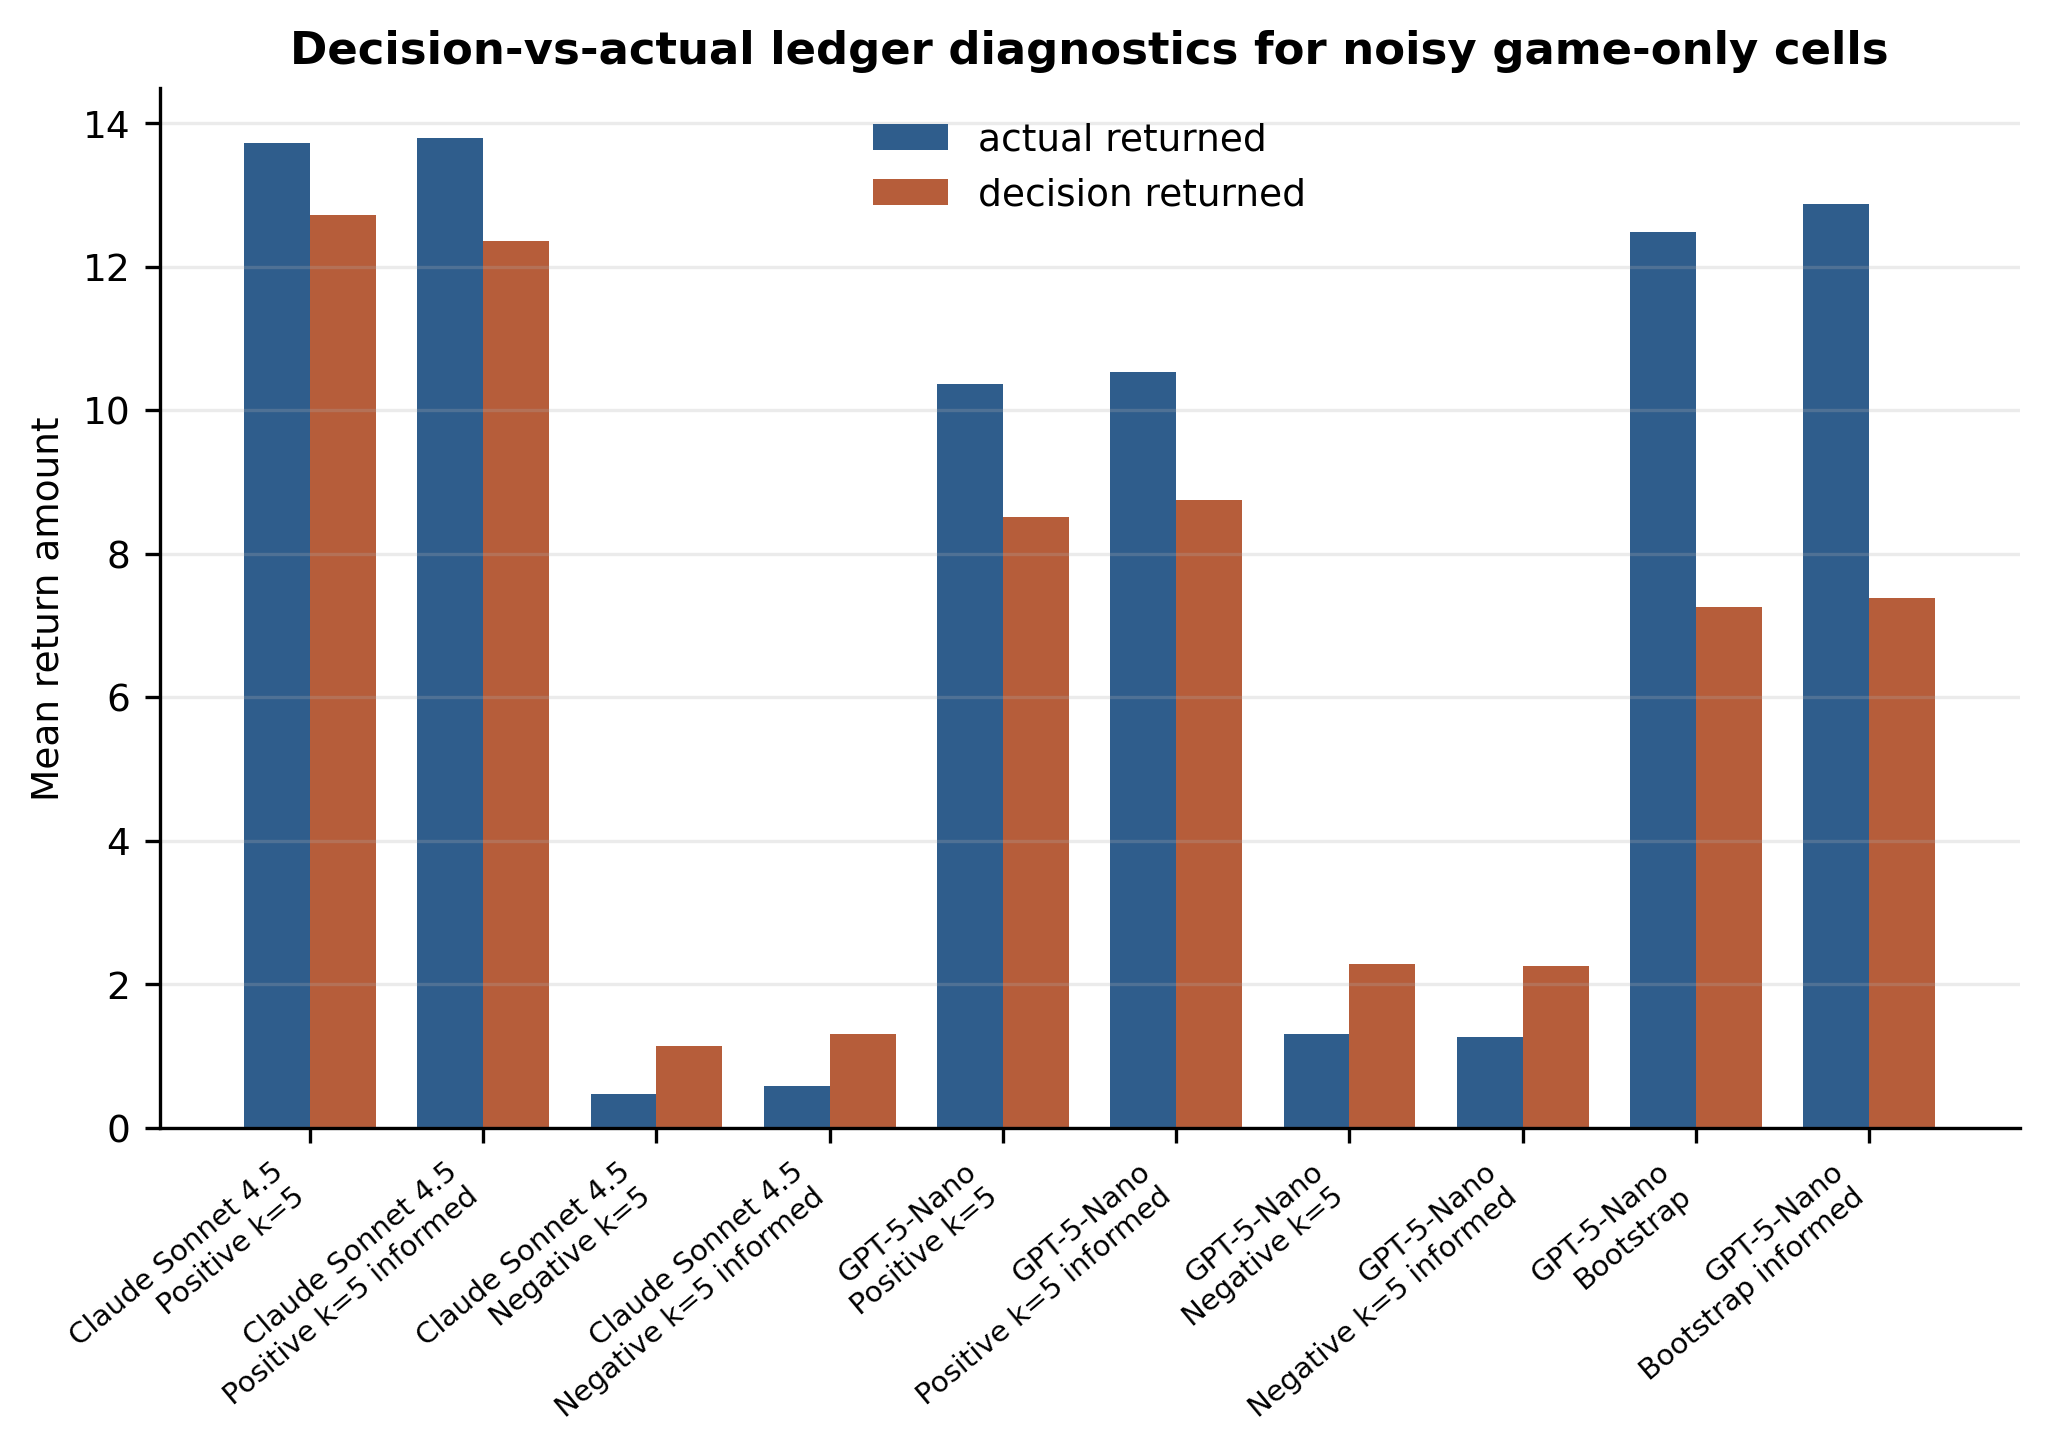
\includegraphics[width=1\linewidth,height=\textheight,keepaspectratio]{figures/appendix_decision_vs_actual.png}

}

\caption{\label{fig-appendix-decision}Decision-vs-actual returned
amounts in noisy game-only cells. The separation is largest when
environmental perturbations or bootstrap returns move the ledger away
from the model's requested return.}

\end{figure}%

\begin{figure}

\centering{

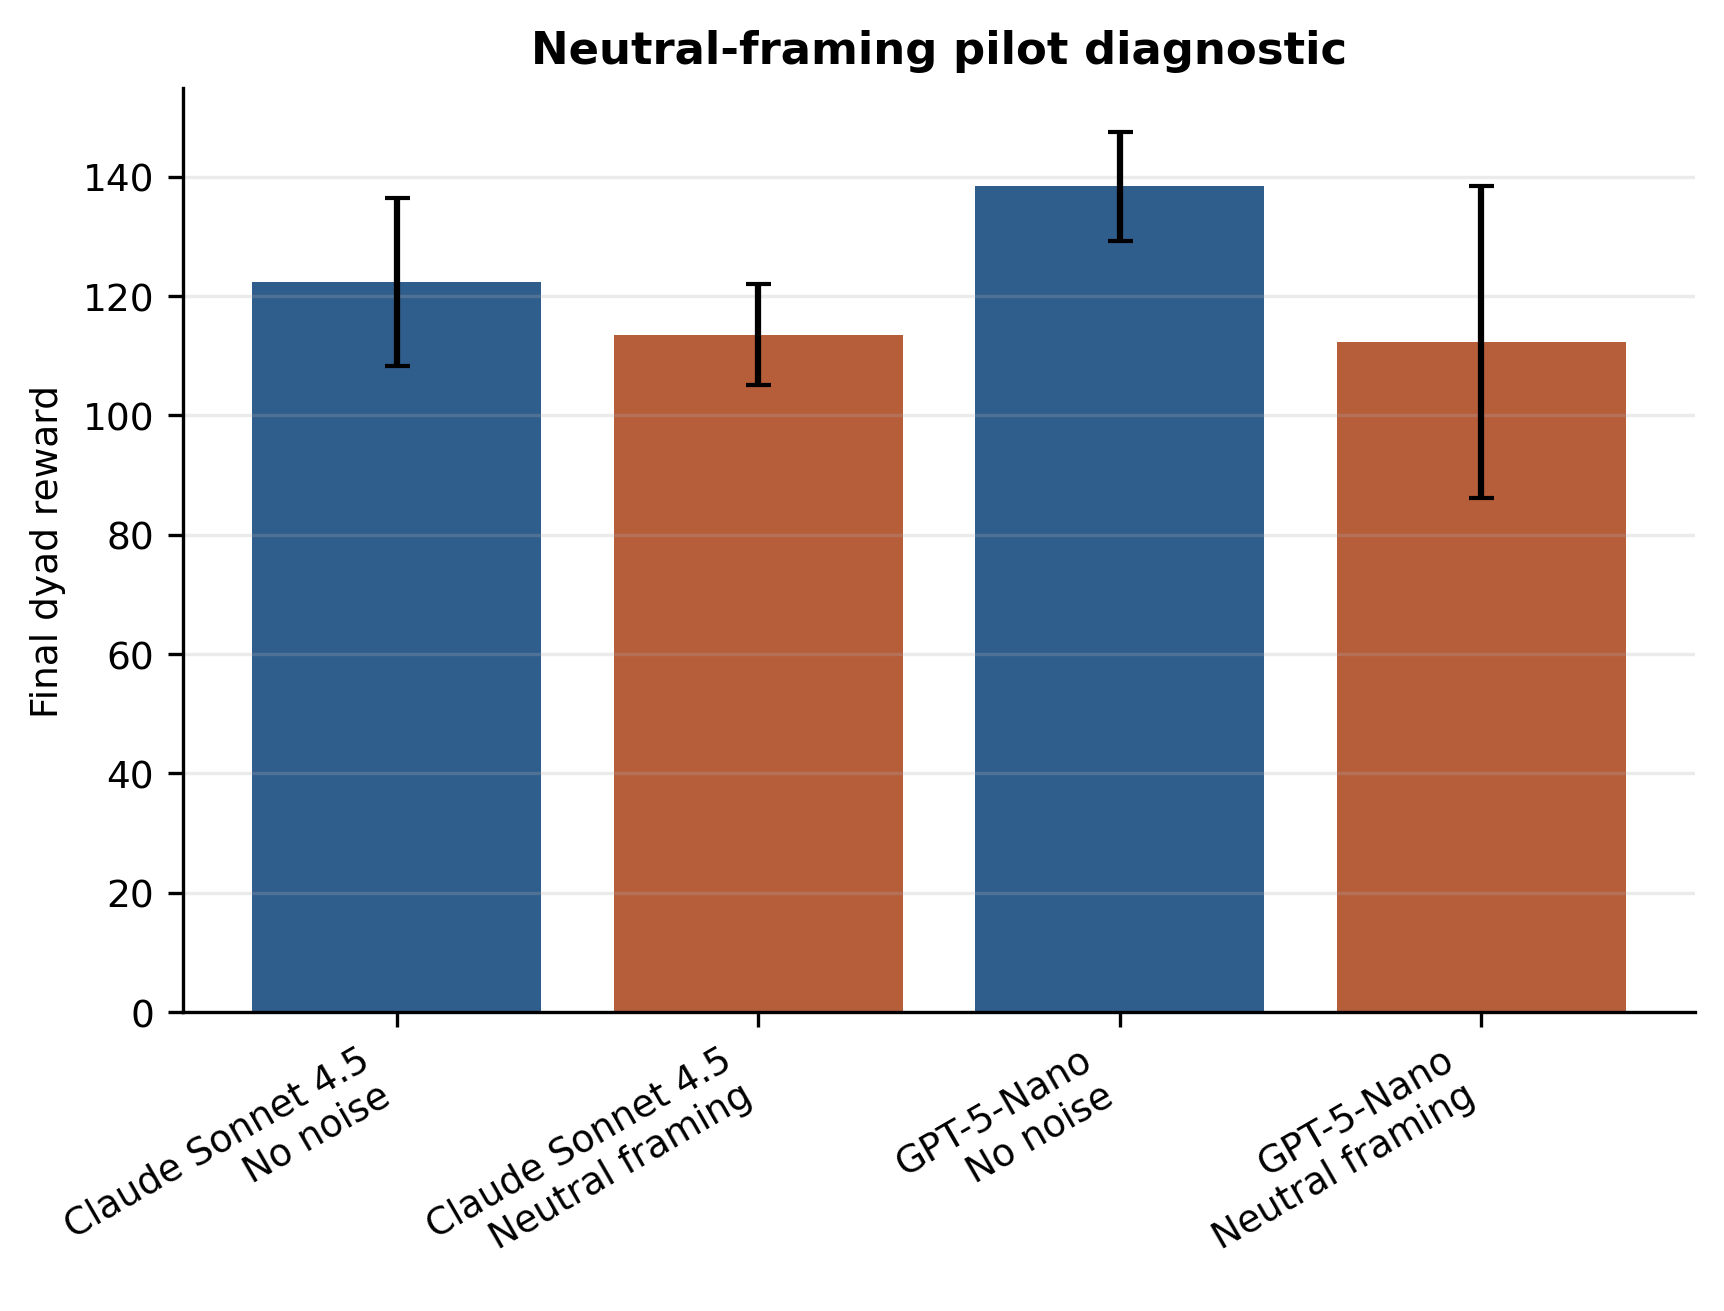
\includegraphics[width=1\linewidth,height=\textheight,keepaspectratio]{figures/appendix_neutral_framing.png}

}

\caption{\label{fig-appendix-neutral}Neutral-framing sanity check:
behavioural distributions under the neutral prompt are equivalent to
those under the standard prompt across matched cells.}

\end{figure}%

\subsection{A.4 Per-cell delta summary (main 24-cell
analysis)}\label{a.4-per-cell-delta-summary-main-24-cell-analysis}

Table A.1 summarises the per-cell mean shift and variance-ratio
estimates for the 24 evaluable (model x noise x myth-order) cells of the
main §4.3 analysis: 4 baseline (no-noise) cells plus 20 noise cells,
excluding one GPT-5-Nano deterministic-max cell
(\(n_{\text{myth}} = 7\), classified as missing). \(\Delta\)mean is the
difference between the matched myth-present cell and its game-only
baseline; var ratio is the across-seed variance ratio (myth/game). 95\%
bootstrap CIs use 2000 resamples. Classifications follow the joint
mean-shift x variance-ratio rule described in §3.5.

\begin{longtable}[]{@{}
  >{\raggedright\arraybackslash}p{(\linewidth - 10\tabcolsep) * \real{0.1667}}
  >{\raggedright\arraybackslash}p{(\linewidth - 10\tabcolsep) * \real{0.1667}}
  >{\raggedright\arraybackslash}p{(\linewidth - 10\tabcolsep) * \real{0.1667}}
  >{\raggedright\arraybackslash}p{(\linewidth - 10\tabcolsep) * \real{0.1667}}
  >{\raggedright\arraybackslash}p{(\linewidth - 10\tabcolsep) * \real{0.1667}}
  >{\raggedright\arraybackslash}p{(\linewidth - 10\tabcolsep) * \real{0.1667}}@{}}
\caption{Per-cell \(\Delta\)mean and variance-ratio estimates (with 95\%
bootstrap CIs) for the main §4.3
analysis.}\label{tbl-percell-deltas}\tabularnewline
\toprule\noalign{}
\begin{minipage}[b]{\linewidth}\raggedright
Model
\end{minipage} & \begin{minipage}[b]{\linewidth}\raggedright
Noise
\end{minipage} & \begin{minipage}[b]{\linewidth}\raggedright
Task order
\end{minipage} & \begin{minipage}[b]{\linewidth}\raggedright
\(\Delta\)mean (95\% CI)
\end{minipage} & \begin{minipage}[b]{\linewidth}\raggedright
Var ratio (95\% CI)
\end{minipage} & \begin{minipage}[b]{\linewidth}\raggedright
Class
\end{minipage} \\
\midrule\noalign{}
\endfirsthead
\toprule\noalign{}
\begin{minipage}[b]{\linewidth}\raggedright
Model
\end{minipage} & \begin{minipage}[b]{\linewidth}\raggedright
Noise
\end{minipage} & \begin{minipage}[b]{\linewidth}\raggedright
Task order
\end{minipage} & \begin{minipage}[b]{\linewidth}\raggedright
\(\Delta\)mean (95\% CI)
\end{minipage} & \begin{minipage}[b]{\linewidth}\raggedright
Var ratio (95\% CI)
\end{minipage} & \begin{minipage}[b]{\linewidth}\raggedright
Class
\end{minipage} \\
\midrule\noalign{}
\endhead
\bottomrule\noalign{}
\endlastfoot
claude & no-noise & game-\textgreater myth & -2.13 {[}-6.34, +2.00{]} &
0.52 {[}0.16, 1.01{]} & null \\
claude & no-noise & myth-\textgreater game & -0.93 {[}-5.14, +3.53{]} &
0.62 {[}0.33, 1.10{]} & null \\
claude & positive & game-\textgreater myth & +1.11 {[}+0.29, +1.96{]} &
0.27 {[}0.02, 1.76{]} & lift \\
claude & positive & myth-\textgreater game & +0.80 {[}-0.13, +1.75{]} &
0.49 {[}0.09, 3.30{]} & null \\
claude & positive (inf) & game-\textgreater myth & +0.59 {[}+0.21,
+0.96{]} & 0.31 {[}0.03, 0.66{]} & lift+consolidation \\
claude & positive (inf) & myth-\textgreater game & +0.15 {[}-0.33,
+0.61{]} & 1.06 {[}0.36, 2.13{]} & null \\
claude & negative\_5 & game-\textgreater myth & +1.29 {[}-1.60, +4.16{]}
& 0.79 {[}0.19, 2.66{]} & null \\
claude & negative\_5 & myth-\textgreater game & +2.48 {[}-0.36, +5.08{]}
& 0.61 {[}0.22, 2.07{]} & null \\
claude & negative\_5 (inf) & game-\textgreater myth & +1.18 {[}-1.26,
+3.33{]} & 0.36 {[}0.13, 1.62{]} & null \\
claude & negative\_5 (inf) & myth-\textgreater game & +1.51 {[}-0.98,
+3.93{]} & 0.67 {[}0.21, 3.00{]} & null \\
gpt5-nano & no-noise & game-\textgreater myth & +1.87 {[}-0.60, +4.33{]}
& 0.36 {[}0.06, 1.78{]} & null \\
gpt5-nano & no-noise & myth-\textgreater game & +3.07 {[}+0.87, +5.33{]}
& 0.06 {[}0.02, 0.23{]} & lift+consolidation \\
gpt5-nano & positive & game-\textgreater myth & +1.65 {[}-0.20, +3.97{]}
& 0.07 {[}0.01, 0.65{]} & consolidation \\
gpt5-nano & positive & myth-\textgreater game & +2.08 {[}+0.26, +4.52{]}
& 0.05 {[}0.00, 0.50{]} & lift+consolidation \\
gpt5-nano & positive (inf) & game-\textgreater myth & +2.23 {[}+0.99,
+3.57{]} & 0.08 {[}0.01, 0.25{]} & lift+consolidation \\
gpt5-nano & positive (inf) & myth-\textgreater game & +1.86 {[}+0.37,
+3.41{]} & 0.50 {[}0.02, 2.19{]} & lift \\
gpt5-nano & negative\_5 & game-\textgreater myth & +4.35 {[}-0.56,
+9.00{]} & 0.39 {[}0.10, 1.09{]} & null \\
gpt5-nano & negative\_5 & myth-\textgreater game & +2.20 {[}-2.80,
+7.19{]} & 0.48 {[}0.18, 1.46{]} & null \\
gpt5-nano & negative\_5 (inf) & game-\textgreater myth & +3.37 {[}-0.65,
+7.20{]} & 1.41 {[}0.62, 3.58{]} & null \\
gpt5-nano & negative\_5 (inf) & myth-\textgreater game & +2.70 {[}-0.81,
+6.23{]} & 0.98 {[}0.41, 2.73{]} & null \\
gpt5-nano & bootstrap & game-\textgreater myth & -7.73 {[}-14.07,
-1.13{]} & 2.09 {[}0.72, 15.95{]} & harmful \\
gpt5-nano & bootstrap & myth-\textgreater game & -7.60 {[}-13.33,
-1.73{]} & 1.46 {[}0.49, 10.76{]} & harmful \\
gpt5-nano & bootstrap (inf) & game-\textgreater myth & -9.67 {[}-14.60,
-4.53{]} & 7.50 {[}3.62, 16.21{]} & destabilizing \\
gpt5-nano & bootstrap (inf) & myth-\textgreater game & -6.87 {[}-11.13,
-2.93{]} & 4.76 {[}1.45, 11.18{]} & destabilizing \\
\end{longtable}

\subsection{A.5 Breadth of partner-myth injection (A1) across
cells}\label{a.5-breadth-of-partner-myth-injection-a1-across-cells}

The A1 effect is regime-conditional rather than uniform. Across all
eight GPT-5-Nano noise cells, A1 produces no detectable behavioural
shift in the positive or negative\_5 cells (\(\Delta\)mean within
\(\pm\) 0.9), and only the bootstrap cells show a substantial
\(\Delta\)mean of approximately +9.3 (Figure~\ref{fig-a1-breadth}). This
pattern situates the rescue described in §4.6 as a property of the
bootstrap regime specifically, not a generic lift from added
partner-related text.

\begin{figure}

\centering{

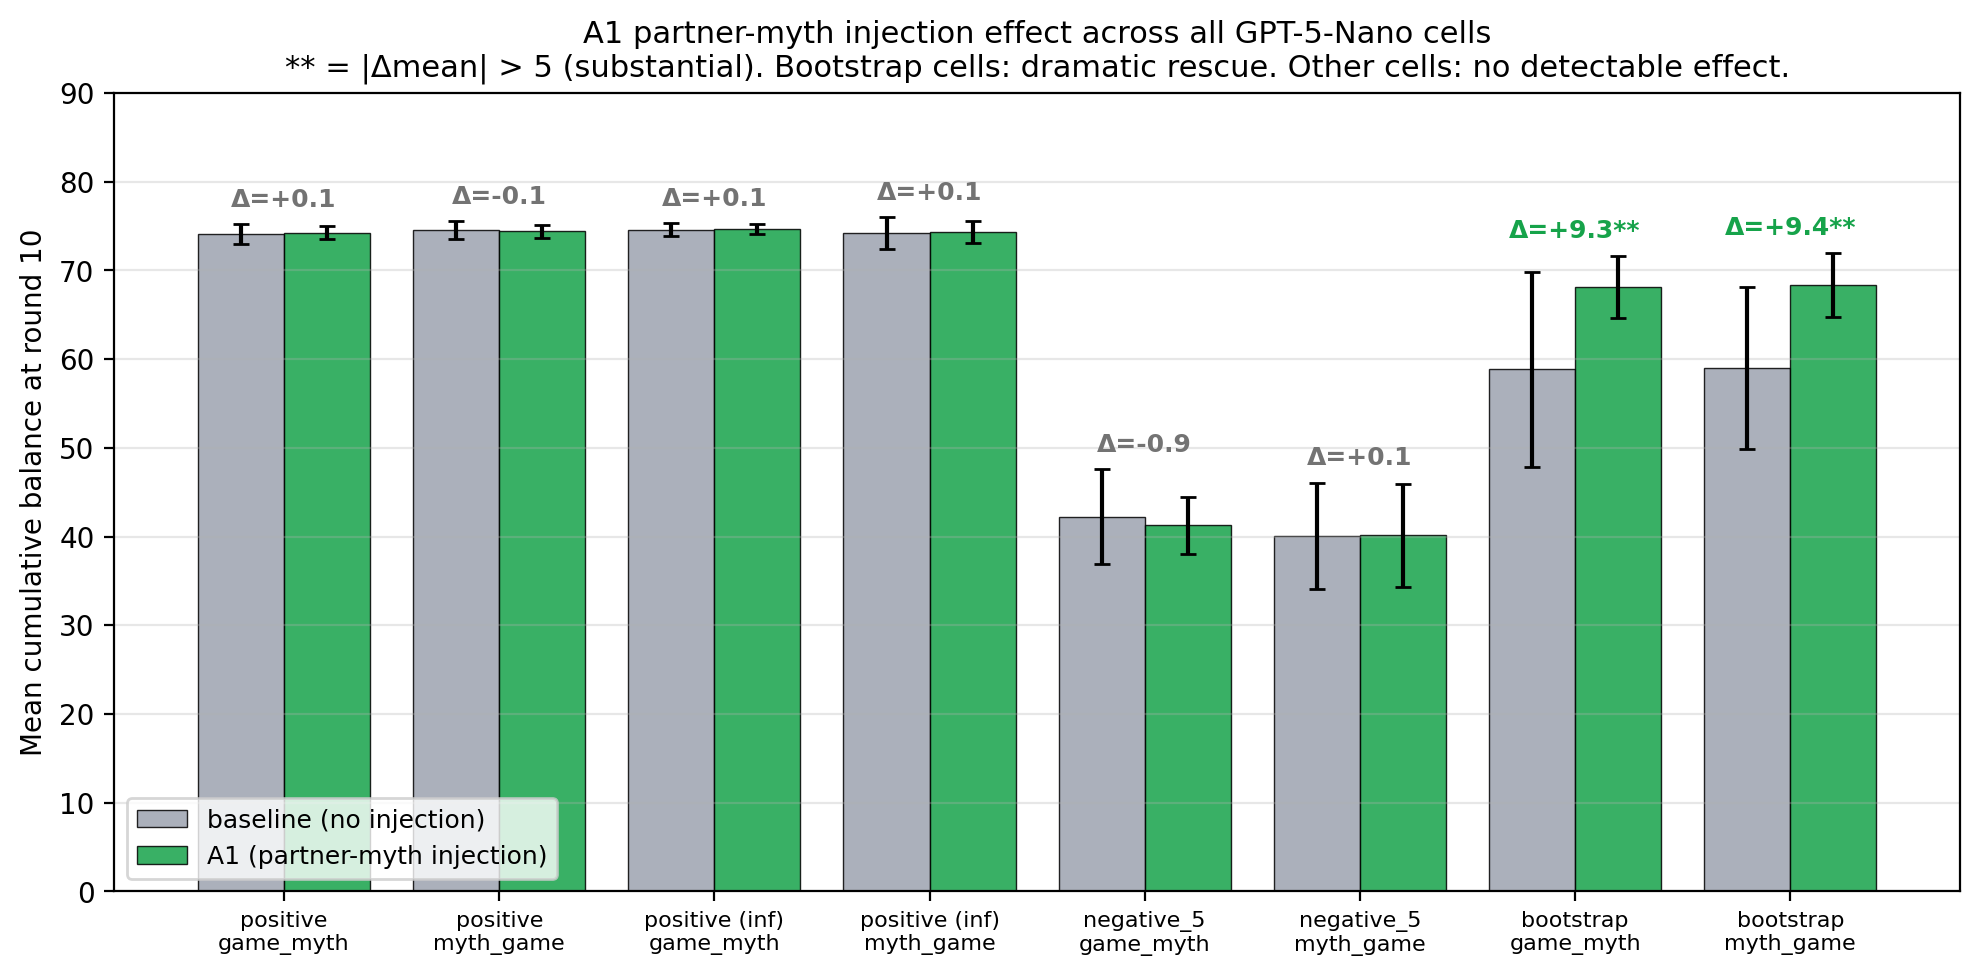
\includegraphics[width=1\linewidth,height=\textheight,keepaspectratio]{figures/fig_a1_deltas.png}

}

\caption{\label{fig-a1-breadth}A1 (partner-myth injection) Delta-mean
across all eight GPT-5-Nano noise cells; the rescue is concentrated in
bootstrap cells and absent in positive and negative\_5 cells.}

\end{figure}%

\subsection{A.6 Deferred analyses}\label{a.6-deferred-analyses}

The current draft omits three analyses that should be added before a
stronger later-conference submission. First, embedding-based myth
similarity should replace lexical Jaccard as the main semantic
convergence measure. Second, a blinded qualitative codebook should
classify recurring myth motifs and explicit reciprocity language. Third,
lagged behavioural models should test whether myth features at round
\(t\) predict send and return decisions at round \(t+1\) after
controlling for the previous game ledger.

\subsection{A.7 Prompt templates}\label{a.7-prompt-templates}

The exact prompts live in \texttt{config/experiments\_noisy.yaml}. For a
submission supplement, copy the system prompt, the four trust-game round
prompts, and the two myth-writing prompts verbatim from that file,
together with the exact experiment-set names used for the final
manifest.


\bibliography{references}

\end{document}
